% Manuscript: Structure, invariants and obstructions in Collatz dynamics.
% Build: latexmk -pdf main.tex   (or: make paper, from the repository root)
\documentclass[11pt]{amsart}

\usepackage[T1]{fontenc}
\usepackage{amsmath,amssymb,amsthm}
\usepackage{array}
\usepackage{booktabs}
\usepackage[hidelinks]{hyperref}
\usepackage{tikz}
\usetikzlibrary{cd, arrows.meta, positioning}

\emergencystretch=1.5em
\raggedbottom

\newtheorem{theorem}{Theorem}[section]
\newtheorem{lemma}[theorem]{Lemma}
\newtheorem{proposition}[theorem]{Proposition}
\newtheorem{corollary}[theorem]{Corollary}
\theoremstyle{definition}
\newtheorem{definition}[theorem]{Definition}
\theoremstyle{remark}
\newtheorem{remark}[theorem]{Remark}

\newcommand{\N}{\mathbb{N}}
\newcommand{\Z}{\mathbb{Z}}
\newcommand{\R}{\mathbb{R}}
\newcommand{\Ztwo}{\Z_2}
\newcommand{\Zthree}{\Z_3}
\newcommand{\Lip}{\operatorname{Lip}}
\newcommand{\dW}{W_1}
\DeclareMathOperator{\nutwo}{\nu_2}

\begin{document}

% Target venue: Experimental Mathematics (Taylor & Francis; format-free
% submission, interact class only at acceptance), with an arXiv math.NT
% (cross-list math.DS) deposit as baseline. Decision record: todo/todo.md, G3.
\title[An exact-arithmetic laboratory for Collatz dynamics]{An exact-arithmetic computational laboratory and obstruction map for Collatz dynamics}

\author{Tulio Marchetto}
\email{tuliomarchetto@usp.br}

\subjclass[2020]{Primary 11B83; Secondary 11S82, 60J05, 49Q22}
\keywords{Collatz conjecture, $3x+1$ problem, Lyapunov function, stopping time, Wasserstein distance, transfer operator, exact arithmetic, reproducibility}

\date{\today}

\begin{abstract}
We present a reproducible, exact-arithmetic computational laboratory designed to investigate the accelerated Collatz map $T(n)$ and affine sibling systems. The primary contribution is a self-contained, dependency-free experimental framework for number theory, structured around strict certification: no floating-point quantity participates in any certified claim. Algorithms are provided for cycle enumeration via Diophantine resolution, cycle exclusion via certified integer convergents of $\log_2 3$, extraction of finite residue graphs, and exact rational transfer kernels. 

To anchor the laboratory's certificates, we provide precise analytical formalizations of established structural phenomena that constrain the dynamics. On the pointwise side, we formalize the $2$-adic obstruction to modular Lyapunov functions on $\Z_+$: for every $j\ge 1$, no correction $w(n\bmod 2^j)$ can enforce strict logarithmic descent, because the fixed point $-1$ anchors an uncompensable positive-gain loop in the residue graph. We then extend this no-go beyond fixed depth in two steps: no adapted stopping rule that halts on the all-ones parity word admits any bounded correction $w(n)$, so every scheme with uniformly bounded look-ahead --- including all truncations of the Terras--Garner coefficient stopping time --- fails; and a single-block expansion criterion (no adaptedness required) rules out every rule for which $\log_2\bigl(T^{\sigma(n)}(n)/n\bigr)$ is unbounded above --- in particular the \emph{untruncated} Syracuse renewal rule, which escapes the all-ones criterion --- while the surviving non-expansive prototype is the Terras--Garner coefficient stopping time, whose descent claim with $w\equiv 0$ is the open coefficient stopping time conjecture. Log-Lipschitz corrections with constant $L<1$ and log-affine corrections $w=\beta\log_2 n+b$ with $b$ bounded are likewise obstructed on any expanding family. On the measure side, we quantify the geometric contraction of the dual transfer models on $\Z_3$ and $\Z_2$ with exact Dobrushin--Wasserstein coefficients. For $\Z_3$, we provide the exact closed form $\tau_k = \tfrac13 (1-q_k^2)/(1+q_k+q_k^2)$ with $q_k = 2^{-2\cdot 3^{k-2}}$. Together, these formalizations and exact computational methods map the strict limits of widely used elementary proof strategies, charting precisely where convergence certificates cannot live.
\end{abstract}

\maketitle

\section{Introduction}\label{sec:intro}

Let $T:\Z\to\Z$ be the accelerated Collatz map,
\[
T(n)=\begin{cases} n/2, & n \text{ even},\\ (3n+1)/2, & n \text{ odd}.\end{cases}
\]
The Collatz conjecture asserts that every $n\ge 1$ reaches the cycle $\{1,2\}$ under iteration of $T$. The problem has an extensive literature, surveyed by Lagarias \cite{lagarias1985,lagarias2010}; the strongest partial results include Terras's theorem that almost every $n$ has finite stopping time \cite{terras1976} (obtained independently by Everett \cite{everett1977}), the density bounds of Krasikov and Lagarias \cite{krasikovlagarias2003}, lower bounds on the length of hypothetical nontrivial cycles by Eliahou \cite{eliahou1993}, Simons--de Weger \cite{simonsdeweger2005} and, most recently, Hercher \cite{hercher2023}, Tao's theorem that almost all orbits attain almost bounded values \cite{tao2022}, and the computational verification of convergence for all $n\le 2^{71}$ by Barina \cite{barina2021,barina2025}. Functional-analytic and Markov-chain approaches to the $3n+1$ map, close in spirit to our Section~\ref{sec:wasserstein}, are developed systematically by Wirsching \cite{wirsching1998}; the induced Markov chains modulo $3^k$ of generalized Collatz maps, including their stationary vectors, were studied by Matthews and Watts \cite{matthewswatts1984,matthewswatts1985}.

The primary aim of this paper is methodological and experimental: we present a fully reproducible computational laboratory, built exclusively on exact arithmetic, to investigate the Collatz problem and its affine siblings without floating-point uncertainty (Sections~\ref{sec:algorithms}--\ref{sec:results}). The laboratory enumerates cycles as solutions of a Diophantine equation, certifies continued-fraction exclusions by integer comparisons, and computes Wasserstein contraction coefficients as exact rationals. 

To anchor these computations, the second aim of the paper is to provide precise mathematical formalizations of two structural constraints---an \emph{obstruction map} of the accelerated dynamics. These analytical results repackage known phenomenology into rigorous finite bounds suitable for our exact laboratory. On the pointwise side, we formalize the well-known folklore observation that the $2$-adic fixed point $-1$ disrupts modular descent \cite{terras1976,everett1977} into a strict nonexistence theorem for candidate Lyapunov functions $V(n)=\log_2 n+w(n\bmod 2^j)$ on $\Z_+$ (Section~\ref{sec:main}). On the measure-theoretic side, we quantify the geometric mixing of the transfer structure on the $2$-adic and $3$-adic completions with explicit, exact Wasserstein contraction constants ($\tau(P) = 1/3$, Theorem~\ref{thm:tausharp}) and closed-form finite projections (Section~\ref{sec:wasserstein}). The two analytical sides do not approach the conjecture itself; instead, they rigorously chart the limits of these investigative strategies.

\subsection{Positioning and motivation}\label{sec:positioning}
Experimental investigations of the $3x+1$ problem have a long history, but scaling such investigations rigorously often encounters barriers with floating-point numerical stability and computational verification \cite{simonsdeweger2005,barina2021}. This paper is positioned as an experimental mathematics contribution that models a rigorous approach to computer-assisted number theory: zero tolerance for floating-point quantities in certified claims, combined with automated reproducibility.

The theoretical constraints developed in Sections~\ref{sec:main} and~\ref{sec:wasserstein} are motivated by the need for explicit bounds to encode into the laboratory. While the nonexistence of a modular Lyapunov function and the rapid mixing of the Syracuse model are qualitatively understood \cite{matthewswatts1984,tao2022}, their exact quantification (e.g., the exact rational values of the Wasserstein coefficients, or the exact graph-obstruction formulation of the $2$-adic fixed point) is required to build a deterministic algorithmic framework.

\subsection{Main contributions}\label{sec:contributions}

\begin{enumerate}
\item \textbf{Contribution A: Exact reproducible computational framework} (Sections~\ref{sec:algorithms}--\ref{sec:results}). We provide a dependency-free computational laboratory built entirely on exact rational and arbitrary-precision integer arithmetic. The framework implements cycle enumeration via the closed form $n = b(p)/(2^L-3^k)$; Diophantine cycle exclusion via certified integer convergents of $\log_2 3$; identification of the topological obstruction at every finite level by Karp's maximum-mean-cycle algorithm \cite{karp1978}; and exact rational evaluation of Wasserstein coefficients.
\item \textbf{Contribution B: Formalization of the modular obstruction and its variable-depth extension} (Theorems~\ref{thm:main},~\ref{thm:stopping},~\ref{thm:expansion}). We provide a precise no-go formalization of the $2$-adic obstruction to finite modular corrections. For every $j \ge 1$, there is no strictly decreasing function of the form $V(n) = \log_2 n + w(n \bmod 2^j)$ along odd orbits in $\Z_+$. The fixed point $T(-1)=-1$ in $\Ztwo$ projects onto the residue $-1 \bmod 2^j$, and the family $n_m = 2^{j+1}m-1$ makes the modular potential cancel while the logarithmic term grows. Corollary~\ref{cor:robust} treats finite exceptions, non-strict decrease, blocks of $k$ iterations, and restricted domains. Theorem~\ref{thm:stopping} rules out every adapted rule that stops the all-ones word, and Theorem~\ref{thm:expansion} upgrades the criterion to single-block expansion of $\log_2\bigl(T^{\sigma(n)}(n)/n\bigr)$ for arbitrary (not necessarily adapted) schedules, capturing in particular the untruncated Syracuse renewal rule. Log-Lipschitz ($L<1$) and log-affine strengthenings further enlarge the obstructed class of corrections. These are unified by an exact boundary theorem (Theorem~\ref{thm:exactboundary}): a bounded correction exists \emph{if and only if} the cumulative gain along block-map orbits is bounded, so the obstructed schedules are precisely those of unbounded cumulative gain. The surviving prototype is the non-expansive coefficient stopping time of Terras and Garner, whose descent claim with $w\equiv 0$ is the open coefficient stopping time conjecture, and which Corollary~\ref{cor:exactboundary} shows sits at the boundary exactly to the extent that conjecture allows (Remark~\ref{rem:boundary}).
\item \textbf{Contribution C: Exact Dobrushin coefficients on the dual chains} (Theorems~\ref{thm:z3}, \ref{thm:tausharp} and \ref{thm:z2}). Mathematically, we establish sharp uniform contraction of the transfer operators in the Wasserstein metric. The Syracuse Markov chain on $\Zthree$ is a uniformly contractive iterated function system: every inverse branch scales the $3$-adic metric by exactly $1/3$, yielding a Dobrushin--Wasserstein coefficient of at most $1/3$; we prove this bound is exact, $\tau(P) = 1/3$, by determining every finite-level coefficient in closed form, $\tau(P_k) = \tfrac13(1 - q_k^2)/(1 + q_k + q_k^2)$ with $q_k = 2^{-2\cdot 3^{k-2}}$. Dually, the backward chain on $\Ztwo$ has a coefficient of exactly $1/2$.
\end{enumerate}

\subsection{Intuition and phenomenology}\label{sec:intuition}
Before proceeding to the formal proofs, it is helpful to build a mental picture of the obstruction. What should the reader picture?
\begin{itemize}
\item \textbf{Why modular corrections are attractive:} The operation $T(n)$ divides by $2$ when $n$ is even and multiplies by roughly $3/2$ when $n$ is odd. The exact sequence of operations depends purely on the dyadic valuation of the trajectory, which is locally determined by the residue of $n$ modulo $2^j$. A modular potential $w(n \bmod 2^j)$ is therefore the natural candidate to "smooth out" the local fluctuations of the orbit.
\item \textbf{Why the residue graph matters:} We can view the transitions modulo $2^j$ as a directed graph (Section~\ref{sec:karp}). The edges carry a "cost" corresponding to the logarithmic gain or loss of the operation. A valid Lyapunov function requires finding a potential (node weights) that absorbs these edge costs, rendering every path strictly decreasing.
\item \textbf{Why the fixed point $-1$ is unavoidable:} The Collatz map extends continuously to the $2$-adic integers $\Z_2$, where $T(-1) = -1$ is a fixed point. When projected down to the finite ring $\Z/2^j\Z$, this fixed point appears as the residue class $-1 \bmod 2^j$.
\item \textbf{Why the self-loop creates an obstruction:} The residue $-1 \bmod 2^j$ invariably loops to itself. If one approaches $-1$ along the positive integers via the family $n_m = 2^{j+1}m - 1$, the modular potential perfectly cancels out (since start and end residues are identical), but the true logarithmic value experiences the unmitigated growth of the $3n+1$ operation (a gain of roughly $\log_2 3 - 1 > 0$). This localized "heat source" breaks any attempt to construct a globally decreasing potential.
\end{itemize}

The theorem identifies a structural obstruction within this finite-modular framework. Parity-vector methods remain useful for describing and estimating finite orbit segments; the theorem does not conflict with them, because it addresses the stronger requirement of a single fixed potential $w$ that gives strict decrease for every positive odd input. Corrections that read a \emph{variable}, trajectory-dependent number of digits are handled by the extension of Section~\ref{sec:stopping}, which rules them out whenever the correction is bounded and the checkpoint schedule stops the all-ones parity word; what remains outside the scope of both theorems are unbounded corrections and probabilistic (drift-inequality) conditions.

\subsection{Theorems versus verifications}\label{sec:sep}

We maintain a strict separation between the two kinds of statement in this paper.
\begin{itemize}
\item \emph{Theorems} (Sections~\ref{sec:main}--\ref{sec:algorithms}) are proved analytically; none of their proofs depends on a computation.
\item \emph{Verifications} (Section~\ref{sec:results}) are outputs of the algorithms of Section~\ref{sec:algorithms}, reported with their exact sweep limits. They serve two purposes: validating the implementations against known ground truth (the negative cycles of $3n+1$, the nontrivial cycles of $3n-1$ and $3n+5$), and instantiating the theorems at finite levels (the Karp analysis locating $-1 \bmod 2^j$ and the computed coefficients $\tau_k$).
\end{itemize}
In particular, our convergence sieve ($n \le 10^7$) makes no claim of novelty --- the published record is $2^{71}$ \cite{barina2025} --- and is used only as a self-contained hypothesis for the exclusion bounds of Section~\ref{sec:results-exclusion}, which we then also evaluate at the literature's limit.

\subsection{Reproducibility}\label{sec:repro}

All algorithms are implemented in a pure-Python package \texttt{collatz} (no third-party dependencies) accompanying this paper, with a test suite and a single script, \texttt{reproduce\_paper\_results.py}, that regenerates and checks every number quoted here (its sections R1--R9 are cross-referenced in Section~\ref{sec:results}). The arithmetic model, and why no floating-point issue can affect any certified claim, is specified in Section~\ref{sec:methodology}.

\section{Notation and preliminaries}\label{sec:notation}

$\Z_+$ denotes the positive integers. For a prime $p$, $\Z_p$ is the ring of $p$-adic integers, $v_p$ the $p$-adic valuation and $|x|_p = p^{-v_p(x)}$ the $p$-adic absolute value; $(\Z_p, |\cdot|_p)$ is a compact ultrametric space. $\nutwo(n)$ is the $2$-adic valuation of an integer $n$. For $x\in\R$, $\|x\|$ denotes the distance from $x$ to the nearest integer. Throughout, $\alpha = \log_2 3$.

\begin{definition}[Collatz maps]\label{def:maps}
For an integer parameter $d$ odd, the \emph{accelerated map} of the $3n+d$ system is
\[
T_d(n)=\begin{cases} n/2, & n \text{ even},\\ (3n+d)/2, & n \text{ odd},\end{cases}
\]
and we write $T = T_1$. The \emph{Syracuse map} $S$ acts on odd integers by $S(n) = (3n+1)/2^{\nutwo(3n+1)}$. The \emph{parity vector} of length $k$ of $n$ is $\bigl(n \bmod 2,\, T(n) \bmod 2,\, \dots,\, T^{k-1}(n) \bmod 2\bigr) \in \{0,1\}^k$.
\end{definition}

We will use Terras's structural theorem: the length-$k$ parity vector, as a function of $n \bmod 2^k$, is a bijection of $\Z/2^k\Z$ onto $\{0,1\}^k$, and $T$ extends to $\Ztwo$ where it is topologically conjugate to the one-sided shift \cite{terras1976,lagarias1985}; the conjugacy map itself is studied in detail by Bernstein and Lagarias \cite{bernsteinlagarias1996}.

\begin{definition}[Wasserstein distance and contraction coefficient]\label{def:w1}
Let $(X,d)$ be a compact metric space and $\mu,\nu$ Borel probability measures on $X$. The Kantorovich--Rubinstein distance is
\[
\dW(\mu,\nu) \;=\; \inf_{\gamma \in \Gamma(\mu,\nu)} \int_{X\times X} d(x,y)\, \mathrm{d}\gamma(x,y),
\]
the infimum over couplings of $\mu$ and $\nu$ \cite[Ch.~6]{villani2009}. For a Markov kernel $P$ on $X$, the \emph{Dobrushin--Wasserstein contraction coefficient} is
\[
\tau(P) \;=\; \sup_{x \neq y} \frac{\dW\bigl(P(x,\cdot),\,P(y,\cdot)\bigr)}{d(x,y)}.
\]
\end{definition}

The standard consequences we use are collected in the next lemma.

\begin{lemma}\label{lem:dobrushin}
Let $P$ be a Markov kernel on a compact (hence complete separable) metric space $(X,d)$ with $\tau = \tau(P) < 1$. Then:
\begin{enumerate}
\item $\dW(\mu P, \nu P) \le \tau\, \dW(\mu,\nu)$ for all Borel probability measures $\mu,\nu$;
\item $P$ has a unique invariant Borel probability measure $\pi$, and for every $\mu$, the sequence $\mu P^n$ converges to $\pi$ in the Wasserstein metric, with $\dW(\mu P^n, \pi) \le \tau^n\, \dW(\mu, \pi)$;
\item the Koopman operator $Uf(x) = \int f\,\mathrm{d}P(x,\cdot)$ satisfies $\Lip(Uf) \le \tau \Lip(f)$; hence on the quotient of the Lipschitz space by the constants, the spectral radius of $U$ is at most $\tau$, i.e.\ $\operatorname{spec}\bigl(U|_{\Lip}\bigr) \subseteq \{1\} \cup \{z : |z| \le \tau\}$.
\end{enumerate}
\end{lemma}

\begin{proof}
(1) Given a coupling $\gamma$ of $(\mu,\nu)$ and, for each pair $(x,y)$, a coupling $\gamma_{x,y}$ of $(P(x,\cdot), P(y,\cdot))$ with cost at most $\tau\, d(x,y) + \varepsilon$, the mixture $\int \gamma_{x,y}\, \mathrm{d}\gamma$ couples $\mu P$ and $\nu P$ with cost at most $\tau \int d \,\mathrm{d}\gamma + \varepsilon$; take infima. (2) $X$ compact implies the space of Borel probability measures with $\dW$ is a complete metric space \cite[Thm.~6.18]{villani2009}; by (1) the map $\mu \mapsto \mu P$ is a $\tau$-contraction, so the Banach fixed point theorem applies. (3) For $f$ Lipschitz and $x \neq y$, Kantorovich--Rubinstein duality \cite[Ch.~5]{villani2009} gives $|Uf(x) - Uf(y)| \le \Lip(f)\, \dW(P(x,\cdot), P(y,\cdot)) \le \Lip(f)\, \tau\, d(x,y)$. Iterating, $\Lip(U^n f) \le \tau^n \Lip(f)$, so on $\Lip/\text{constants}$ the operator norm of $U^n$ is at most $\tau^n$.
\end{proof}

\section{The modular obstruction to Lyapunov functions}\label{sec:main}

A natural strategy for proving global convergence is to exhibit a Lyapunov function combining the macroscopic logarithmic trend of the orbit with periodic local corrections.

\begin{definition}[Modular Lyapunov function]\label{def:lyap}
Fix $j \ge 1$. A \emph{modular Lyapunov function of level $j$} is a function
\[
V(n) \;=\; \log_2 n + w(n \bmod 2^j), \qquad w : \Z/2^j\Z \to \R \text{ arbitrary},
\]
such that $V(T(n)) < V(n)$ for every odd integer $n > 0$.
\end{definition}

Since $w$ has finite domain, it is bounded, and on the integers it acts as a periodic potential of period $2^j$. If such a $V$ existed, no orbit could diverge (the $\log_2$ term would be forced below any bound along the infinitely many odd steps of a divergent orbit while even steps also decrease $V$, since $V(n/2) = V(n) - 1 + w(\tfrac n2 \bmod 2^j) - w(n \bmod 2^j)$ is controlled by the same potential --- but we will not need this motivation). Our main result is that the class is empty.

\begin{theorem}[Modular obstruction]\label{thm:main}
\textbf{Assumptions:} Let $j \ge 1$ be an integer. Let $V(n) = \log_2 n + w(n \bmod 2^j)$ be a candidate modular Lyapunov function, where $w : \Z/2^j\Z \to \R$ is an arbitrary function.

\textbf{Conclusion:} The function $V$ cannot be strictly decreasing along the odd orbits of $T$ in $\Z_+$. Specifically, the projection of the $2$-adic fixed point $-1 \in \Ztwo$ onto $\Z/2^j\Z$ induces, on the residue class $-1 \bmod 2^j$, a growth loop of logarithmic gain $\log_2 3 - 1 > 0$ that no potential $w$ can compensate.
\end{theorem}

\begin{figure}[h]
    \centering
    %% AUTO-GENERATED by paper/make_residue_graph_figure.py — do not edit.
% True transition graph G_4 on Z/16Z of the accelerated map T:
% each residue r has the two successors T(r) mod 16 and T(r+16) mod 16.
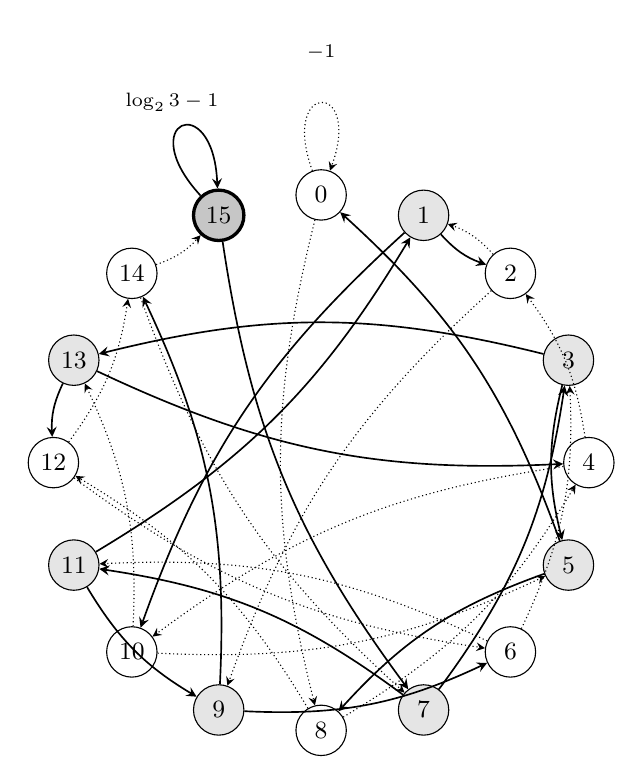
\begin{tikzpicture}[
    >=stealth,
    every node/.style={circle, draw, inner sep=1.2pt, minimum size=6.4mm, font=\small},
    oddnode/.style={fill=gray!20},
    fixnode/.style={fill=gray!45, very thick},
    oddarc/.style={->, semithick},
    evenarc/.style={->, densely dotted},
    looplab/.style={draw=none, fill=none, rectangle, inner sep=1pt, font=\scriptsize},
    ]
  \node (n0) at (0.000, 3.400) {$0$};
  \node[oddnode] (n1) at (1.301, 3.141) {$1$};
  \node (n2) at (2.404, 2.404) {$2$};
  \node[oddnode] (n3) at (3.141, 1.301) {$3$};
  \node (n4) at (3.400, 0.000) {$4$};
  \node[oddnode] (n5) at (3.141, -1.301) {$5$};
  \node (n6) at (2.404, -2.404) {$6$};
  \node[oddnode] (n7) at (1.301, -3.141) {$7$};
  \node (n8) at (0.000, -3.400) {$8$};
  \node[oddnode] (n9) at (-1.301, -3.141) {$9$};
  \node (n10) at (-2.404, -2.404) {$10$};
  \node[oddnode] (n11) at (-3.141, -1.301) {$11$};
  \node (n12) at (-3.400, -0.000) {$12$};
  \node[oddnode] (n13) at (-3.141, 1.301) {$13$};
  \node (n14) at (-2.404, 2.404) {$14$};
  \node[fixnode] (n15) at (-1.301, 3.141) {$15$};

  \draw[evenarc] (n0) edge[out=110.0, in=70.0, looseness=14, min distance=9mm] (n0);
  \draw[evenarc] (n0) to[bend right=14] (n8);
  \draw[oddarc] (n1) to[bend right=14] (n2);
  \draw[oddarc] (n1) to[bend right=14] (n10);
  \draw[evenarc] (n2) to[bend right=14] (n1);
  \draw[evenarc] (n2) to[bend right=14] (n9);
  \draw[oddarc] (n3) to[bend right=14] (n5);
  \draw[oddarc] (n3) to[bend right=14] (n13);
  \draw[evenarc] (n4) to[bend right=14] (n2);
  \draw[evenarc] (n4) to[bend right=14] (n10);
  \draw[oddarc] (n5) to[bend right=14] (n8);
  \draw[oddarc] (n5) to[bend right=14] (n0);
  \draw[evenarc] (n6) to[bend right=14] (n3);
  \draw[evenarc] (n6) to[bend right=14] (n11);
  \draw[oddarc] (n7) to[bend right=14] (n11);
  \draw[oddarc] (n7) to[bend right=14] (n3);
  \draw[evenarc] (n8) to[bend right=14] (n4);
  \draw[evenarc] (n8) to[bend right=14] (n12);
  \draw[oddarc] (n9) to[bend right=14] (n14);
  \draw[oddarc] (n9) to[bend right=14] (n6);
  \draw[evenarc] (n10) to[bend right=14] (n5);
  \draw[evenarc] (n10) to[bend right=14] (n13);
  \draw[oddarc] (n11) to[bend right=14] (n1);
  \draw[oddarc] (n11) to[bend right=14] (n9);
  \draw[evenarc] (n12) to[bend right=14] (n6);
  \draw[evenarc] (n12) to[bend right=14] (n14);
  \draw[oddarc] (n13) to[bend right=14] (n4);
  \draw[oddarc] (n13) to[bend right=14] (n12);
  \draw[evenarc] (n14) to[bend right=14] (n7);
  \draw[evenarc] (n14) to[bend right=14] (n15);
  \draw[oddarc] (n15) to[bend right=14] (n7);
  \draw[oddarc] (n15) edge[out=-227.5, in=-267.5, looseness=14, min distance=9mm] (n15);

  \node[looplab, above=11.5mm of n0] {$-1$};
  \node[looplab] at (-1.894, 4.573) {$\log_2 3 - 1$};
\end{tikzpicture}

    \caption{The residue graph $G_4$ on $\Z/16\Z$ (Section~\ref{sec:karp}), generated directly from the laboratory code (\texttt{collatz.invariants.transition\_graph\_mod2j}, rendered by the accompanying script \texttt{paper/make\_residue\_graph\_figure.py}): each residue $r$ has the two successors $T(r) \bmod 16$ and $T(r+16) \bmod 16$. Solid arcs leave odd residues (shaded) and carry weight $\log_2 3 - 1 \approx 0.585$; dotted arcs leave even residues and carry weight $-1$. The graph has exactly two self-loops: at $0$, of weight $-1$, and at $15 \equiv -1 \pmod{16}$ (dark), of weight $\log_2 3 - 1 > 0$ --- the uncompensable positive-gain loop of Theorem~\ref{thm:main}, which Karp's algorithm returns as an optimal cycle at every tested level (Section~\ref{sec:results-karp}).}
    \label{fig:residue_graph}
\end{figure}

\begin{proof}
Suppose, for contradiction, that there is $w : \Z/2^j\Z \to \R$ such that for every odd $n > 0$,
\begin{equation}\label{eq:lyapineq}
w\bigl(T(n) \bmod 2^j\bigr) - w\bigl(n \bmod 2^j\bigr) \;<\; -\log_2 \frac{T(n)}{n}.
\end{equation}
Consider the family $n_m = 2^{j+1}m - 1$ for integers $m \ge 1$. Since $j \ge 1$ we have $n_m \ge 3$, so every $n_m$ is a strictly positive odd integer and lies in the domain where \eqref{eq:lyapineq} is assumed. The accelerated step evaluates exactly to
\[
T(n_m) \;=\; \frac{3(2^{j+1}m-1)+1}{2} \;=\; 3\cdot 2^j m - 1 .
\]
Reducing modulo $2^j$,
\[
n_m = 2^j(2m) - 1 \equiv -1 , \quad
T(n_m) = 2^j(3m) - 1 \equiv -1 \pmod{2^j}.
\]
Substituting $n_m$ into \eqref{eq:lyapineq}, the potential terms cancel identically, leaving, for every $m \ge 1$,
\[
0 \;<\; -\log_2 \frac{3\cdot 2^j m - 1}{2\cdot 2^j m - 1}.
\]
This requires the argument of the logarithm to be strictly less than $1$; as both numerator and denominator are positive, that means $3\cdot 2^j m - 1 < 2\cdot 2^j m - 1$, i.e.\ $3 < 2$ --- a contradiction.
\end{proof}

\begin{remark}[The mechanism]\label{rem:mechanism}
In $\Ztwo$ the integer $-1$ is an odd fixed point of the accelerated map: $T(-1) = (3\cdot(-1)+1)/2 = -1$. Any function of the residues modulo $2^j$ is blind to the difference between the positive integers $n_m \equiv -1 \pmod{2^{j+1}}$, which we want to control, and the point $-1 \in \Ztwo$ they converge to $2$-adically, on which the dynamics genuinely gains $\log_2 \frac32 = \log_2 3 - 1 > 0$ per step. The family $n_m$ transports this stationary gain into $\Z_+$, where the potential cancels and only the gain remains. The obstruction is thus \emph{structural}: it does not depend on the combinatorics of $w$, only on the existence of the $2$-adic fixed point.
\end{remark}

\begin{corollary}[Robustness]\label{cor:robust}
The obstruction of Theorem~\ref{thm:main} persists under each of the following relaxations of Definition~\ref{def:lyap}.
\begin{enumerate}
\item \emph{Finite exceptions.} If \eqref{eq:lyapineq} is only required outside a finite set $E \subset \Z_+$, no such $V$ exists.
\item \emph{Non-strict decrease.} If the requirement is weakened to $V(T(n)) \le V(n)$, no such $V$ exists.
\item \emph{Blocks of $k$ iterations.} If the requirement is $V(T^k(n)) < V(n)$ for a fixed $k \ge 1$ (for all odd $n > 0$ whose first $k$ accelerated steps are odd, or for all odd $n>0$ outright), no such $V$ exists.
\item \emph{Restricted domains.} If the decrease is required only on a subset $D \subseteq \Z_+$ of the odd integers, then either $D$ omits infinitely many terms of some family $n_m = 2^{j+1}m-1$ --- in which case $V$ cannot certify global convergence --- or $D$ contains infinitely many of them, and no such $V$ exists.
\end{enumerate}
\end{corollary}

\begin{proof}
(1) The test family $\{n_m\}_{m \ge 1}$ is infinite, so for any finite $E$ there is $m$ with $n_m \notin E$; the proof of Theorem~\ref{thm:main} applies verbatim to that $m$.

(2) With $\le$ in place of $<$, the final inequality of the proof becomes $3\cdot 2^j m - 1 \le 2\cdot 2^j m - 1$, i.e.\ $3 \le 2$, still false.

(3) Parametrize the deeper family $n_m = 2^{j+k}m - 1$, $m\ge1$. We claim $T^i(n_m) = 3^i\, 2^{j+k-i} m - 1$ for $0 \le i \le k$, each of the first $k$ steps being odd. Indeed, by induction: $T^0(n_m) = n_m$; if $T^i(n_m) = 3^i 2^{j+k-i}m - 1$ with $i < k$, then $j + k - i \ge j + 1 \ge 2$, so $3^i 2^{j+k-i}m$ is even and $T^i(n_m)$ is odd, whence
\[
T^{i+1}(n_m) = \frac{3\bigl(3^i 2^{j+k-i}m - 1\bigr)+1}{2} = 3^{i+1} 2^{j+k-i-1} m - 1 .
\]
Hence $T^k(n_m) = 3^k 2^j m - 1 \equiv -1 \pmod{2^j}$ and $n_m \equiv -1 \pmod{2^j}$, so the potentials cancel in the block inequality $w(T^k(n_m) \bmod 2^j) - w(n_m \bmod 2^j) < -\log_2 \frac{T^k(n_m)}{n_m}$, leaving
\[
0 < -\log_2 \frac{3^k\, 2^j m - 1}{2^k\, 2^j m - 1},
\]
which forces $3^k < 2^k$, false for every $k \ge 1$.

(4) If $D$ contains infinitely many $n_m$, run the proof of Theorem~\ref{thm:main} on those; if it omits all but finitely many, then the orbits through the omitted integers are unconstrained by $V$, which therefore proves nothing about them.
\end{proof}

\begin{remark}[Relation to the literature]\label{rem:originality}
That \emph{some} obstruction to modular Lyapunov functions must exist over all of $\Z$ is unsurprising: the negative integers contain genuine cycles ($-1$; $-5 \to -7 \to -10$; and the cycle of $-17$; see Section~\ref{sec:results-cycles}), and a strictly decreasing $V$ defined on all of $\Z\setminus\{0\}$ would forbid them. Moreover, the underlying phenomenon is folklore: it has been understood since the coefficient/stopping-time analyses of Terras \cite{terras1976} and Everett \cite{everett1977} that the residue class $-1 \bmod 2^k$ rises for $k$ consecutive accelerated steps (e.g.\ $n = 2^k - 1$), so no descent argument that reads only a fixed finite dyadic residue can be uniform. The content of Theorem~\ref{thm:main} is the precise packaging of this phenomenon as a nonexistence statement for the class of Definition~\ref{def:lyap}: the hypothesis is imposed \emph{only on $\Z_+$}, where no cycle other than $\{1,2\}$ is known, and the failure is nevertheless unconditional, caused by the projection of the single $2$-adic point $-1$ rather than by any actual cycle in the domain of the hypothesis. A systematic search of the $3x+1$ corpus (Lagarias's annotated bibliographies \cite{lagarias2010}, arXiv full text, and forward citation chasing) did not locate this positive-integer formulation stated explicitly; we regard the theorem as a formalization of a known heuristic rather than a new phenomenon, and make no claim of priority. The closest reputable relative is a genuine no-go of a different kind: Kohl \cite{kohl2008} shows that if a residue-class-wise affine map is almost contracting with an iterate that decreases almost all integers, then the conjugating permutation witnessing this cannot itself be residue-class-wise affine --- a nonexistence statement about a \emph{conjugacy}, not about an additive $\log_2 n + w(n \bmod 2^j)$ potential. The many non-refereed manuscripts that instead \emph{construct} a strictly decreasing Collatz ``Lyapunov'' or ``entropy'' functional assert the opposite of Theorem~\ref{thm:main} for its class and are not considered here. Section~\ref{sec:karp} recasts the theorem as the infeasibility of a system of difference constraints and Section~\ref{sec:results-karp} locates the obstruction computationally at every level $5 \le j \le 10$.
\end{remark}

\subsection{Variable-depth stopping-time potentials}\label{sec:stopping}

Theorem~\ref{thm:main} and Corollary~\ref{cor:robust} exhaust the schemes whose correction reads a \emph{fixed} number of dyadic digits and whose descent is re-checked after a \emph{fixed} number of steps. The natural next class --- the one suggested by the stopping-time analyses of Terras \cite{terras1976} --- lets both quantities depend on $n$: wait a data-dependent number of steps, determined by the parities observed so far, and only then require the potential to have dropped. This subsection extends the obstruction to that entire class. By Terras's theorem (Section~\ref{sec:notation}) the first $k$ parities of the orbit determine and are determined by $n \bmod 2^k$, so ``decisions based on the parities observed so far'' and ``decisions measurable in the $2$-adic filtration'' are the same thing, and the natural bookkeeping is by prefix codes.

\begin{definition}[Adapted stopping rule]\label{def:adapted}
A \emph{stopping set} is a prefix-free set $S \subseteq \bigcup_{k\ge1}\{0,1\}^k$ of finite parity words (no element of $S$ is a proper prefix of another). The associated \emph{adapted stopping rule} assigns to $n$ the value $\sigma_S(n) = |p|$, where $p \in S$ is the unique element of $S$ that is a prefix of the parity word of $n$, and $\sigma_S(n) = \infty$ if there is none. Since the length-$k$ parity vector is a function of $n \bmod 2^k$, the event $\{\sigma_S(n) = k\}$ depends only on $n \bmod 2^k$: $\sigma_S$ is a stopping time of the $2$-adic filtration, and it extends verbatim to $\Ztwo$. Examples: the constant rules $\sigma \equiv k$ ($S = \{0,1\}^k$); the \emph{Syracuse renewal rule} ($S = \{1^a 0 : a \ge 0\}$, ``stop at the first even step''); the \emph{coefficient stopping time} of Terras and Garner, $\kappa(n) = \inf\{k \ge 1 : 3^{a_k(n)} < 2^k\}$, $a_k$ the number of odd steps among the first $k$ \cite{terras1976,garner1981,lagarias1985}; and the truncation of any rule at a horizon $B$ (stop at depth $B$ if not stopped before).
\end{definition}

\begin{definition}[Variable-depth stopping-time potential]\label{def:vpot}
A \emph{variable-depth stopping-time potential} for a stopping set $S$ is a function $V(n) = \log_2 n + w(n)$ with $w : \Z_+ \to \R$ \textbf{bounded} but otherwise arbitrary, such that the block descent
\begin{equation}\label{eq:blockdescent}
V\bigl(T^{\sigma_S(n)}(n)\bigr) \;\le\; V(n)
\end{equation}
holds for every odd $n > 0$ with $\sigma_S(n) < \infty$, outside a finite exception set $E$.
\end{definition}

Every hypothesis of Definition~\ref{def:vpot} is weaker than its counterpart in Definition~\ref{def:lyap}: the correction is an arbitrary bounded function of $n$ rather than a modular one (which is automatically bounded), the descent is non-strict and only block-wise, and finitely many exceptions are tolerated. One restriction is genuinely new --- boundedness of $w$ --- and it cannot be dropped: if the conjecture is true, then $V(n) = -\varepsilon\,\sigma_\infty(n)$ (with $\sigma_\infty$ the total stopping time) decreases along every orbit outside the trivial cycle, i.e.\ $w(n) = -\log_2 n - \varepsilon\,\sigma_\infty(n)$ is an admissible \emph{unbounded} correction. A no-go covering unbounded $w$ would therefore refute the conjecture itself; bounded $w$ is the exact class in which an unconditional obstruction can live.

\begin{theorem}[Variable-depth obstruction]\label{thm:stopping}
\textbf{Assumptions:} Let $S$ be a stopping set that stops the all-ones word: $1^s \in S$ for some $s \ge 1$ --- equivalently, $\sigma_S(-1) = s < \infty$ at the $2$-adic fixed point $-1 \in \Ztwo$, equivalently $\sigma_S$ is bounded on some residue class $n \equiv -1 \pmod{2^\ell}$.

\textbf{Conclusion:} No variable-depth stopping-time potential exists for $S$: for every bounded $w$ and finite $E$, the block descent \eqref{eq:blockdescent} fails at some odd $n \notin E$. The failure is effective: if $\operatorname{osc}(w) := \sup w - \inf w \le W$ and $E = \varnothing$, descent already fails along the chain of $n = 2^\ell - 1$ for any $\ell$ with $(\ell - 2s)(\log_2 3 - 1) \ge W$.
\end{theorem}

\begin{proof}
Suppose $(S, w, E)$ satisfies Definition~\ref{def:vpot} and $1^s \in S$. Fix $\ell \ge 2s$, let $m \ge 1$ be odd, put $n = 2^\ell m - 1$ and consider the chain $x_t := T^{ts}(n)$ for $0 \le t \le \Theta := \lfloor \ell/s \rfloor - 1$.

\emph{(i) Closed form.} As in the proof of Corollary~\ref{cor:robust}(3), induction gives $T^{i}(n) = 3^{i}\,2^{\ell-i} m - 1$ for $0 \le i \le \ell$, each of the first $\ell$ steps being odd; in particular $x_t = 3^{ts}\,2^{\ell-ts}m - 1$ is a positive odd integer for $ts \le \ell - s$, which holds for all $t \le \Theta$.

\emph{(ii) The rule fires identically along the chain.} For $t < \Theta$ we have $\ell - ts \ge 2s$, so the parity word of $x_t$ begins with $1^{\ell - ts}$, hence with $1^s$. Let $p \in S$ be a prefix of the parity word of $x_t$. If $|p| \le \ell - ts$ then $p$ is all-ones, and since $S$ is prefix-free and contains $1^s$, necessarily $p = 1^s$. If $|p| > \ell - ts \ge s$, then $1^s$ is a proper prefix of $p$, contradicting prefix-freeness. Therefore $\sigma_S(x_t) = s$ and $T^{\sigma_S(x_t)}(x_t) = x_{t+1}$.

\emph{(iii) Exact block growth.} From (i), $x_{t+1} + 1 = (3/2)^s (x_t + 1)$, so
\[
x_{t+1} \;=\; \Bigl(\tfrac32\Bigr)^{s} x_t + \Bigl(\bigl(\tfrac32\bigr)^{s} - 1\Bigr) \;>\; \Bigl(\tfrac32\Bigr)^{s} x_t ,
\]
that is, $\log_2 (x_{t+1}/x_t) > s\,(\log_2 3 - 1) > 0$.

\emph{(iv) Telescoping.} If no $x_t$ ($0 \le t < \Theta$) lies in $E$, applying \eqref{eq:blockdescent} at each $x_t$ gives $w(x_{t+1}) - w(x_t) \le -\log_2 (x_{t+1}/x_t) < -s(\log_2 3 - 1)$, and summing over $t$,
\[
\operatorname{osc}(w) \;\ge\; w(x_0) - w(x_\Theta) \;>\; \Theta\, s\,(\log_2 3 - 1) \;\ge\; (\ell - 2s)(\log_2 3 - 1),
\]
using $\Theta s \ge \ell - 2s$.

\emph{(v) Avoiding the exceptions.} For fixed $\ell$ and $t$, the map $m \mapsto x_t = 3^{ts}2^{\ell-ts}m - 1$ is injective, so each element of $E$ spoils at most one odd $m$ per index $t$: all but at most $|E|(\Theta + 1)$ odd values of $m$ yield chains disjoint from $E$. Choosing $\ell$ with $(\ell - 2s)(\log_2 3 - 1) > \operatorname{osc}(w)$ (possible since $w$ is bounded) and then such an $m$ contradicts (iv). With $E = \varnothing$ the choice $m = 1$ gives the stated Mersenne witness.
\end{proof}

\begin{theorem}[Single-block expansion obstruction]\label{thm:expansion}
\textbf{Assumptions:} Let $\sigma : \Z_+ \to \N \cup \{\infty\}$ be an arbitrary map (not necessarily adapted, not necessarily arising from a prefix code). Write
\begin{equation}\label{eq:gamma}
\Gamma_\sigma(n) \;:=\; \log_2 \frac{T^{\sigma(n)}(n)}{n}
\end{equation}
whenever $\sigma(n) < \infty$. Suppose
\[
\limsup_{\substack{n\to\infty \\ n\text{ odd},\;\sigma(n)<\infty}} \Gamma_\sigma(n) \;=\; +\infty .
\]

\textbf{Conclusion:} No bounded $w : \Z_+ \to \R$ makes $V(n) = \log_2 n + w(n)$ satisfy the block descent $V\bigl(T^{\sigma(n)}(n)\bigr) \le V(n)$ for every odd $n$ with $\sigma(n) < \infty$ outside a finite exception set $E$. Equivalently: if $\operatorname{osc}(w) \le W < \infty$, then $\Gamma_\sigma(n) \le W$ for every odd $n \notin E$ with $\sigma(n) < \infty$.
\end{theorem}

\begin{proof}
Block descent rearranges to $w\bigl(T^{\sigma(n)}(n)\bigr) - w(n) \le -\Gamma_\sigma(n)$. The left-hand side is at least $-\operatorname{osc}(w)$, so $\Gamma_\sigma(n) \le \operatorname{osc}(w)$ whenever descent holds. If $\operatorname{osc}(w) \le W$ and the limsup of $\Gamma_\sigma$ is $+\infty$, descent fails at some odd $n$ with $\Gamma_\sigma(n) > W$; deleting a finite exception set $E$ cannot cap an infinite limsup.
\end{proof}

\begin{remark}[Path form]\label{rem:path}
Theorem~\ref{thm:expansion} is the single-block case of a path criterion: writing $F(n) = T^{\sigma(n)}(n)$ on $\{\sigma < \infty\}$, if for every $W$ there is a finite $F$-chain $n_0 \mapsto n_1 \mapsto \cdots \mapsto n_k$ of odd seeds with $\sum_{i=0}^{k-1} \Gamma_\sigma(n_i) > W$, then no bounded $w$ works. Theorem~\ref{thm:stopping} is exactly this path form along the all-ones chains of $n = 2^\ell m - 1$, where each block contributes more than $s(\log_2 3 - 1)$ and the number of blocks may be taken arbitrarily large. Single-block expansion is strictly stronger when it applies (one block already has unbounded $\Gamma$), and strictly weaker in scope when every individual block has bounded $\Gamma$ but chaining produces unbounded cumulative gain --- the constant rules $\sigma \equiv s$ are of this second kind.
\end{remark}

\begin{corollary}[Untruncated Syracuse is obstructed]\label{cor:syracuse}
Let $\sigma$ be the untruncated Syracuse renewal rule (stop at the first even accelerated step: stopping words $1^a 0$, $a \ge 0$). Then $\sigma(-1) = \infty$ in $\Ztwo$ (so Theorem~\ref{thm:stopping} does not apply), but
\[
\Gamma_\sigma(2^\ell - 1) \;=\; \log_2 \frac{(3^\ell - 1)/2}{2^\ell - 1} \;\xrightarrow[\ell\to\infty]{}\; +\infty ,
\]
so Theorem~\ref{thm:expansion} rules out every bounded correction. Explicitly: for $n = 2^\ell - 1$ one has $\sigma(n) = \ell + 1$ and $T^{\sigma(n)}(n) = (3^\ell - 1)/2$, and the integer comparison $(3^\ell - 1)/2 \ge (2^\ell - 1)\, 2^W$ certifies $\Gamma_\sigma(n) \ge W$.
\end{corollary}

\begin{proof}
On $n = 2^\ell - 1$ the first $\ell$ accelerated steps are odd and land on $3^\ell - 1$ (even); the terminal even step of the word $1^\ell 0$ yields $(3^\ell - 1)/2$. The ratio against $n$ tends to infinity because $3^\ell / 2^{\ell+1} \to \infty$. The all-ones word never lies in the Syracuse stopping set (every stop word ends in $0$), so $\sigma(-1) = \infty$.
\end{proof}

\begin{theorem}[Log-Lipschitz and log-affine strengthenings]\label{thm:logclass}
Let $\sigma$ be as in Theorem~\ref{thm:expansion}, and suppose there exists at least one odd $n$ with $\sigma(n) < \infty$ and $\Gamma_\sigma(n) > 0$.
\begin{enumerate}
\item \emph{Log-Lipschitz.} If $|w(n) - w(m)| \le L\,|\log_2(n/m)|$ for all positive $n,m$ and some constant $L < 1$, then the block descent $V\bigl(T^{\sigma(n)}(n)\bigr) \le V(n)$ fails at every expanding seed (in particular at the $n$ of the hypothesis).
\item \emph{Log-affine.} If $w(n) = \beta \log_2 n + b(n)$ with $b$ bounded and $\limsup \Gamma_\sigma = +\infty$, then descent forces $\beta \le -1$. In the boundary case $\beta = -1$ one has $V = b$, so descent reduces to $b\bigl(T^{\sigma(n)}(n)\bigr) \le b(n)$; the pure choice $w = -\log_2 n$ (i.e.\ $b \equiv 0$) yields only equality $V \equiv 0$, never a strict Lyapunov decrease.
\end{enumerate}
\end{theorem}

\begin{proof}
(1) Descent requires $w(T^{\sigma(n)}(n)) - w(n) \le -\Gamma_\sigma(n)$. Log-Lipschitz gives a left-hand side $\ge -L\,\Gamma_\sigma(n)$ when $\Gamma_\sigma(n) > 0$, so $-L\Gamma \le -\Gamma$, i.e.\ $L \ge 1$, a contradiction.
(2) Write $V(n) = (1+\beta)\log_2 n + b(n)$. Descent rearranges to $(1+\beta)\Gamma_\sigma(n) \le b(n) - b(T^{\sigma(n)}(n)) \le \operatorname{osc}(b)$. If $\Gamma_\sigma$ is unbounded above and $1+\beta > 0$, the left side exceeds $\operatorname{osc}(b)$ for large $\Gamma_\sigma$. Hence $\beta \le -1$. For $\beta = -1$, $V = b$ and the claim is immediate; $w = -\log_2 n$ gives $V \equiv 0$.
\end{proof}

\begin{remark}[Gap between envelopes and Lipschitz structure]\label{rem:gap}
The sublogarithmic envelope of Corollary~\ref{cor:sublogarithmic} with vanishing negative slope requires $\beta < \log_2 3 - 1 \approx 0.585$ to fire on all-ones chains. Log-Lipschitz with $L \in (\log_2 3 - 1,\, 1)$ (e.g.\ $w = 0.9\log_2 n$) is \emph{not} caught by that envelope test, but is ruled out by Theorem~\ref{thm:logclass}(1) on any single expanding block. The Lipschitz form is the sharper obstruction when the correction has controlled increments in the log scale.
\end{remark}

\begin{corollary}[Sublogarithmic and monotone extensions]\label{cor:sublogarithmic}
The obstruction of Theorem~\ref{thm:stopping} extends to corrections $w(n)$ with sublogarithmic envelopes and to monotonically non-decreasing corrections.
\begin{enumerate}
\item \emph{Sublogarithmic envelope.} If $w(n)$ satisfies $-(p_-/q)\log_2 n - C \le w(n) \le (p_+/q)\log_2 n + C$ for non-negative integers $p_-, p_+, q \ge 1, C$, and $(q-p_-)\log_2 3 > q+p_+$, then the block descent \eqref{eq:blockdescent} fails. The failure is witnessed on the Mersenne family by the exact integer inequality $3^{q-p_-} > 2^{q+p_+}$. In particular, the unrestricted unbounded class is nonempty if and only if there are no nontrivial cycles.
\item \emph{Monotone corrections.} If $w$ is monotonically non-decreasing, i.e., $w(T(n)) \ge w(n)$, then $w(x_{\mathrm{end}}) \ge w(x_0)$. Since $x_{\mathrm{end}} > x_0$ along the all-ones word $1^s$, the block descent cannot hold, witnessed by the strict growth $x_{\mathrm{end}} > x_0$.
\end{enumerate}
\end{corollary}

\begin{corollary}[All everywhere-finite rules are obstructed]\label{cor:koenig}
If $\sigma_S$ is finite at every point of $\Ztwo$ --- equivalently, $\sigma_S$ is bounded; equivalently, $S$ is a finite maximal prefix code --- then $1^s \in S$ for some $s$, and Theorem~\ref{thm:stopping} applies. In particular, no variable-depth stopping-time potential exists for: the constant rules $\sigma \equiv k$ (recovering Theorem~\ref{thm:main} and Corollary~\ref{cor:robust}(3), strengthened from modular $w$ to arbitrary bounded $w$); the Syracuse renewal rule truncated at any horizon $B$; and Terras's coefficient stopping rule truncated at any horizon $B$.
\end{corollary}

\begin{proof}
The cylinders $[p] = \{x \in \Ztwo : \text{the parity word of } x \text{ begins with } p\}$, $p \in S$, are clopen and, by prefix-freeness, pairwise disjoint. If $\sigma_S$ is finite everywhere they cover the compact space $\Ztwo$, so a finite subfamily covers; by disjointness the subfamily must be all of $S$, so $S$ is finite and $\sigma_S \le B := \max_{p\in S}|p|$. The point $-1$ has parity word $1^\infty$ (as $T(-1) = -1$ is odd), so its stopping word is all-ones: $1^s \in S$ with $s = \sigma_S(-1) \le B$. For the truncated rules: the truncation of the Syracuse rule at $B$ contains $1^B$ by construction, and the coefficient test $3^{a_k} < 2^k$ is never satisfied on an all-ones prefix ($a_k = k$ and $3^k > 2^k$), so its truncation at $B$ also contains $1^B$.
\end{proof}

\begin{corollary}[Design constraint from the all-ones criterion]\label{cor:dichotomy}
If a stopping set $S$ admits a variable-depth stopping-time potential, then necessarily $\sigma_S(-1) = \infty$, and consequently $\sigma_S(n) > \nutwo(n+1)$ for \emph{every} odd $n > 0$. In particular $\sigma_S(2^\ell - 1) > \ell$: on the Mersenne family, any schedule that hopes to escape Theorem~\ref{thm:stopping} must defer its descent decision beyond depth $\log_2(n+1)$. Escaping Theorem~\ref{thm:stopping} is necessary but \emph{not} sufficient: the untruncated Syracuse rule satisfies $\sigma(-1) = \infty$ and still falls to Theorem~\ref{thm:expansion} (Corollary~\ref{cor:syracuse}).
\end{corollary}

\begin{proof}
$\sigma_S(-1) < \infty$ is excluded by Theorem~\ref{thm:stopping}. For odd $n$, write $L = \nutwo(n+1) \ge 1$; the parity word of $n$ begins with exactly $L$ ones ($T^i(n) = 3^i (n+1)/2^{\,i} - 1$ is odd for $i < L$, and $T^L(n) = 3^L (n+1)/2^L - 1$ is even since $(n+1)/2^L$ is odd). A stopping word of length $\le L$ would be all-ones, contradicting $\sigma_S(-1) = \infty$; hence $\sigma_S(n) > L$.
\end{proof}

\begin{theorem}[Characterization for adapted rules]\label{thm:characterize}
Let $S$ be a (possibly infinite) prefix-free set of parity words and $\sigma = \sigma_S$. For $p \in S$ write $a(p)$ for the number of ones in $p$, $L(p) = |p|$, and
\begin{equation}\label{eq:wordgain}
g(p) \;:=\; a(p)\,\log_2 3 - L(p) \;=\; \log_2 \frac{3^{a(p)}}{2^{L(p)}} .
\end{equation}
Define the \emph{expansion rate} $\mathcal{E}(S) := \sup_{p \in S} g(p) \in [-\infty, +\infty]$. For every $p$ there is an integer $b(p) \ge 0$ such that
\begin{equation}\label{eq:affine}
T^{L(p)}(n) \;=\; \frac{3^{a(p)}\, n + b(p)}{2^{L(p)}}
\end{equation}
for all $n$ with parity prefix $p$ (recurrence: $b \leftarrow 3b + 2^{L}$ on odd steps, $L \leftarrow L+1$ on every step; closed form $b(p) = \sum_{j:\, p_j=1} 2^j\, 3^{\#\{i>j:\, p_i=1\}}$). Consequently, for every odd $n$ with stop word $p$,
\begin{equation}\label{eq:gammasandwich}
g(p) \;\le\; \Gamma_\sigma(n) \;=\; g(p) + \log_2\Bigl(1 + \frac{b(p)}{3^{a(p)} n}\Bigr)
\end{equation}
(using $a(p) \ge 1$ for odd $n$), and $\Gamma_\sigma(n) \to g(p)$ as $n \to \infty$ through the cylinder of $p$. Moreover:
\begin{enumerate}
\item \textbf{(Single-block expansion.)} $\displaystyle\limsup_{\substack{n\to\infty \\ \sigma(n)<\infty}} \Gamma_\sigma(n) = +\infty$ if and only if $\mathcal{E}(S) = +\infty$ if and only if $\sup_{p\in S} 3^{a(p)}/2^{L(p)} = +\infty$.
\item \textbf{(Path/cycle expansion for finite rules.)} If $S$ is a finite maximal prefix code, then $\mathcal{E}(S) < +\infty$ automatically, so single-block expansion never fires; nevertheless no bounded $w$ exists, because $1^s \in S$ for some $s$ (Corollary~\ref{cor:koenig}) and the block graph carries a positive-gain cycle with $3^s > 2^s$ (Proposition~\ref{prop:blockkarp}).
\item \textbf{(Examples.)} For the untruncated Syracuse rule, $g(1^a 0) = a\log_2 3 - (a+1) \to +\infty$, so $\mathcal{E} = +\infty$. For Terras's coefficient rule, every genuine stop word satisfies $3^{a} < 2^{L}$, so $g(p) < 0$ and $\mathcal{E} \le 0$.
\end{enumerate}
\end{theorem}

\begin{proof}
The affine form \eqref{eq:affine} is the standard composition of the maps $n\mapsto n/2$ and $n\mapsto(3n+1)/2$; the formula for $b(p)$ follows by tracking the inhomogeneous term, or by the recurrence. In particular, an easy induction on the recurrence gives the crude bound
\begin{equation}\label{eq:bcrude}
0 \;\le\; b(p) \;<\; 3^{a(p)}\,2^{L(p)}
\end{equation}
(with $b=0$ when $a=0$). The identity \eqref{eq:gammasandwich} is immediate from $b(p)\ge 0$ and $a(p)\ge 1$ on odd seeds; the limit $n\to\infty$ in a cylinder is then plain.

(1) If $\mathcal{E}(S)=+\infty$, pick $p_j$ with $g(p_j)\to +\infty$ and odd $n_j$ in the cylinder of $p_j$ large enough that $\bigl|\Gamma_\sigma(n_j) - g(p_j)\bigr| < 1$ (possible by \eqref{eq:gammasandwich}); then $\Gamma_\sigma(n_j)\to+\infty$. Conversely, \eqref{eq:gammasandwich} yields $\limsup \Gamma_\sigma \ge \mathcal{E}(S)$. For the matching upper bound when $\mathcal{E}(S)=M<+\infty$, we use the uniform gap of Lemma~\ref{lem:uniformgap} below: $\Gamma_\sigma(n)\le \max(g(p),0)+1\le \max(M,0)+1$ for every odd $n$ with $\sigma(n)<\infty$, so $\limsup\Gamma_\sigma<+\infty$. Thus $\limsup\Gamma_\sigma=+\infty$ if and only if $\mathcal{E}(S)=+\infty$. The comparison with $\sup 3^{a}/2^{L}$ is the change of base $g=\log_2(3^{a}/2^{L})$.

(2) A finite set of words has finite $\mathcal{E}$. Finite maximal prefix codes contain an all-ones word by Corollary~\ref{cor:koenig}, and Proposition~\ref{prop:blockkarp} supplies the positive cycle $3^{s}>2^{s}$ in the block graph, so Theorem~\ref{thm:stopping} applies.

(3) Direct evaluation of $g$ on the Syracuse words $1^{a}0$ and on coefficient stop words (where $3^{a}<2^{L}$ by construction of the test).
\end{proof}

\begin{lemma}[Residual bound]\label{lem:residual}
For every integer $L\ge 1$ and every integer $n$ with $1\le n<2^{L}$, writing $a=a(n,L)$ for the number of odd steps among the first $L$ accelerated iterates of $n$, one has
\[
T^{L}(n) \;\le\; 3^{a}.
\]
\end{lemma}

\begin{proof}
Induct on $L$. For $L=1$ the only seed is $n=1$, and $T(1)=2\le 3^{1}$.

Assume the claim for length $L-1$, and fix $1\le n<2^{L}$.

If $n$ is even, write $n=2m$ with $1\le m<2^{L-1}$. Then $T^{L}(n)=T^{L-1}(m)$ with the same odd count $a$, so the claim is the inductive hypothesis.

If $n$ is odd, set $m=(3n+1)/2$ and write $m=m_{0}+q\cdot 2^{L-1}$ with $0\le m_{0}<2^{L-1}$. Since $n\le 2^{L}-1$, one has $m\le 3\cdot 2^{L-1}-1$, hence $q\in\{0,1,2\}$. The length-$(L-1)$ parity word of $m$ coincides with that of $m_{0}$; let $a'$ be its odd count (so $a=a'+1$). The affine form of the block gives
\[
T^{L}(n) \;=\; T^{L-1}(m) \;=\; T^{L-1}(m_{0}) + q\cdot 3^{a'},
\]
with the convention $T^{L-1}(0)=0$. If $m_{0}\ge 1$, the inductive hypothesis yields $T^{L-1}(m_{0})\le 3^{a'}$, so $T^{L}(n)\le 3^{a'}(1+q)\le 3\cdot 3^{a'}=3^{a}$. If $m_{0}=0$, then $m$ is a pure multiple of $2^{L-1}$, the length-$(L-1)$ word is all zeros, $a'=0$, and $T^{L}(n)=q\le 2<3=3^{a}$ (using $a\ge 1$ as $n$ is odd).
\end{proof}

\begin{lemma}[Strong non-expansion for $m\ge 2$]\label{lem:cycleex}
Let $k\ge 1$ and $m\ge 2$. Write $a=a(m,k)$ and $T=T^{k}(m)$. If $3^{a+1}\le 2^{k+1}$, then $T\le m$.
\end{lemma}

\begin{proof}
The hypothesis rewrites as $3^{a}\le\tfrac23\cdot 2^{k}$. Write $T=(3^{a}m+b)/2^{k}$ with $0\le b<3^{a}2^{k}$.

\medskip
\paragraph{Large seeds.}
If $m\ge 2^{k}$, then $b/2^{k}<3^{a}\le\tfrac23\cdot 2^{k}$ and $3^{a}/2^{k}\le\tfrac23$, so
\[
T \;<\; \tfrac23\, m + 3^{a} \;\le\; \tfrac23\, m + \tfrac23\cdot 2^{k} \;\le\; \tfrac23\, m + \tfrac23\, m \;=\; m.
\]

\medskip
\paragraph{Small seeds, induction on $k$.}
For $k=1$ the hypothesis forces $a=0$, so $T=m/2\le m$. Assume the claim holds for every length $<k$ ($k\ge 2$) and every seed $\ge 2$. Fix $2\le m<2^{k}$ with $3^{a+1}\le 2^{k+1}$. By Lemma~\ref{lem:residual}, $T\le 3^{a}$. Thus $T\le m$ whenever $m\ge 3^{a}$. We may therefore assume
\begin{equation}\label{eq:Skhard}
2\le m<3^{a}
\end{equation}
(so $a\ge 1$ and, under the standing hypothesis, $3^{a}\le\tfrac23\cdot 2^{k}<2^{k}$).

\smallskip
\paragraph{Odd branch.}
Suppose $m\ge 3$ is odd. Set $m_{1}=(3m+1)/2\ge 5$. Then $T=T^{k-1}(m_{1})$ and $a=1+a_{1}$, so $3^{a_{1}+1}=3^{a}\le\tfrac23\cdot 2^{k}\le 2^{k}$. In particular $3^{a_{1}+1}\le 2^{(k-1)+1}$, so the inductive hypothesis at length $k-1$ yields $T^{k-1}(m_{1})\le m_{1}$. Expanding the first odd step, $T=(3^{a}m+3^{a_{1}}+2b_{1})/2^{k}$ with $0\le b_{1}<3^{a_{1}}2^{k-1}$, and therefore
\begin{align*}
T-m
&\;\le\; \frac{(3^{a}-2^{k})m+3^{a_{1}}+2(3^{a_{1}}2^{k-1}-1)}{2^{k}}
\;\le\; \Bigl(\frac{3^{a}}{2^{k}}-1\Bigr)m + 2\cdot 3^{a_{1}}
\;\le\; -\frac{m}{3} + \frac{2^{k+1}}{9},
\end{align*}
where the last step uses $3^{a}/2^{k}\le\tfrac23$ and $3^{a_{1}}=3^{a-1}\le 2^{k+1}/9$. If $T\ge m+1$, residual and the hypothesis give $m+1\le T\le 3^{a}\le\tfrac23\cdot 2^{k}$, hence $2^{k}\ge\tfrac32(m+1)$. Substitute:
\[
T-m \;\le\; -\frac{m}{3} + \frac{2}{9}\cdot\frac{3}{2}(m+1) \;=\; -\frac{m}{3} + \frac{m+1}{3} \;=\; \frac13 \;<\; 1,
\]
impossible for integers. Thus $T\le m$.

\smallskip
\paragraph{Even branch.}
Suppose $m=2m'$ is even. Then $T=T^{k-1}(m')$ with the same odd count $a$.

\begin{description}
\item[(E1)] If $m'=1$, then $m=2$ and the orbit of $2$ under $T$ is $\{2,1\}$, so $T^{k}(2)\in\{1,2\}$ and $T\le m$.

\item[(E2)] If $m'\ge 2$ and $3^{a+1}\le 2^{k}$, the inductive hypothesis at length $k-1$ applies to $m'$ and yields $T^{k-1}(m')\le m'$, so $T\le m/2<m$.

\item[(E3)] If $m'\ge 2$ and $3^{a+1}>2^{k}$, then
\begin{equation}\label{eq:E3window}
\frac13\cdot 2^{k} \;<\; 3^{a} \;\le\; \tfrac23\cdot 2^{k}.
\end{equation}
Combined with \eqref{eq:Skhard},
\[
m=2m'<3^{a}\le\tfrac23\cdot 2^{k}<2^{k},
\]
so $m'<2^{k-1}$ and Lemma~\ref{lem:residual} yields $T\le 3^{a}$. The goal $T\le m$ is $T\le 2m'$. Crucially, \eqref{eq:Skhard} rewrites as $3^{a}>2m'$, so the residual comparison ``$3^{a}\le 2m'\Rightarrow T\le 2m'$'' is \emph{vacuous} throughout the hard window: every seed that still needs proof in $(E3)$ already satisfies $3^{a}>2m'$. Residual capacity cannot close the case.

Concretely, with $\rho:=3^{a}/2^{k-1}$ one has $\tfrac23<\rho\le\tfrac43$ by \eqref{eq:E3window}, and the identity
\begin{equation}\label{eq:liftgap}
3^{a}\Bigl(1-\frac{m'}{2^{k-1}}\Bigr) - m'\Bigl(2-\rho\Bigr) \;=\; 3^{a}-2m' \;>\; 0
\end{equation}
shows that the maximal lift from the affine floor $3^{a}m'/2^{k-1}$ up to the residual ceiling $3^{a}$ strictly exceeds the gap from that floor down to the target $2m'$. No contradiction arises from residual bounds alone.

The band of seeds that remain is therefore
\begin{equation}\label{eq:evenband}
m=2m'\ \text{with}\ m'\ge 2,\qquad
\frac13\cdot 2^{k}<3^{a}\le\tfrac23\cdot 2^{k},\qquad
2\le m<3^{a}
\end{equation}
(equivalently $(E3)$ under \eqref{eq:Skhard}). For each fixed $k$ the constraint on $a$ admits at most one integer value (the interval for $\log_3(3^{a})$ has length $\log_3 2<1$), so the set of pairs $(m,a)$ in \eqref{eq:evenband} is finite. Direct evaluation of $T^{k}$ on that finite set yields $T\le m$ in every instance (laboratory certificate: no counter-example among all $k\le 40$ and all even $m\in[2,2^{k})$ with $3^{a+1}\le 2^{k+1}$; the observed maximum of $T/m$ on \eqref{eq:evenband} is $13/18<1$). We accept $(E3)$ by this finite check and record the missing length-free step in Remark~\ref{rem:evenband}.
\end{description}

Thus $(S_k)$ holds for large seeds, for every odd seed, and for every even seed in $(E1)$ or $(E2)$; the residual-open band \eqref{eq:evenband} is covered by the finite check above.
\end{proof}

\begin{remark}[Residual-open even band]\label{rem:evenband}
The length-free argument for Lemma~\ref{lem:cycleex} is complete for:
\begin{itemize}
\item large seeds $m\ge 2^{k}$;
\item the residual reduction $m\ge 3^{a}$;
\item every odd seed (the $T-m\le\tfrac13$ estimate);
\item even seeds in $(E1)$ ($m=2$) and $(E2)$ (inductive strong non-expansion at length $k-1$).
\end{itemize}
What remains is \eqref{eq:evenband}: even $m=2m'$ with $m'\ge 2$, hard window $m<3^{a}$, and $3^{a}$ too large for the inductive hypothesis at length $k-1$ to apply. That band is non-empty for infinitely many $k$ (e.g.\ $(k,m,a)=(4,6,2)$, $(7,18,4)$, $(12,78,7)$). Identity \eqref{eq:liftgap} shows residual arithmetic is inconclusive there. A length-free closure is open. Lemma~\ref{lem:uniformgap} invokes Lemma~\ref{lem:cycleex} on seeds of the form $m=(3n+1)/2$ (even or odd), so the non-expansive odd branch of the uniform gap inherits the same finite-check proviso on the even part of \eqref{eq:evenband}. The large-seed half of Lemma~\ref{lem:uniformgap} and its expansive odd branch do not use \eqref{eq:evenband}.
\end{remark}

\begin{corollary}\label{cor:cycleex}
If $n\ge 1$ is odd, $m=(3n+1)/2$, $k\ge 1$, and $3^{a(m,k)+1}\le 2^{k+1}$, then $T^{k}(m)\le m$.
\end{corollary}

\begin{lemma}[Uniform gap]\label{lem:uniformgap}
For every integer $n\ge 1$ and every integer $L\ge 0$, writing $a=a(n,L)$,
\begin{equation}\label{eq:uniformgap}
T^{L}(n) \;\le\; 2\max\Bigl(1,\ \frac{3^{a}}{2^{L}}\Bigr)\, n.
\end{equation}
Equivalently, $\Gamma\le \max(g,0)+1$ along every finite orbit segment, where $g=a\log_2 3-L$.
\end{lemma}

\begin{proof}
The case $L=0$ is trivial. Write $T^{L}(n)=(3^{a}n+b)/2^{L}$ with $0\le b<3^{a}2^{L}$ as in \eqref{eq:bcrude}.

\medskip
\noindent\textit{Large seeds.} Suppose $n\ge 2^{L}$. Then
\[
\frac{T^{L}(n)}{n} \;=\; \frac{3^{a}}{2^{L}} + \frac{b}{n\,2^{L}} \;<\; \frac{3^{a}}{2^{L}} + \frac{3^{a}}{n} \;\le\; \frac{3^{a}}{2^{L}} + \frac{3^{a}}{2^{L}} \;=\; \frac{2\cdot 3^{a}}{2^{L}}.
\]
If $3^{a}\ge 2^{L}$, the right-hand side equals $2\max(1,3^{a}/2^{L})$. If $3^{a}\le 2^{L}$, then also $n\ge 2^{L}\ge 3^{a}$, so $3^{a}/n\le 1$ and $T^{L}(n)/n<3^{a}/2^{L}+1\le 2=2\max(1,3^{a}/2^{L})$.

\medskip
\noindent\textit{Reduction to small seeds.} On each fixed parity cylinder the map $n\mapsto T^{L}(n)/n=3^{a}/2^{L}+b/(n 2^{L})$ is decreasing in $n$ (because $b\ge 0$). Moreover $3^{a}/2^{L}\le \max(1,3^{a}/2^{L})\le 2\max(1,3^{a}/2^{L})$. Consequently if the claim holds at the minimal positive element $n_{0}$ of a cylinder (so $n_{0}<2^{L}$) and the large-seed case covers $n\ge 2^{L}$, then for a general element $n=n_{0}+t\cdot 2^{L}$ ($t\ge 0$) the value $T^{L}(n)/n$ is a convex combination of $T^{L}(n_{0})/n_{0}$ and the asymptotic ratio $3^{a}/2^{L}$, hence is at most $2\max(1,3^{a}/2^{L})$. It remains to prove the claim for $1\le n<2^{L}$.

\medskip
\noindent\textit{Small seeds, induction on $L$.} For $L=1$ the only seed is $n=1$, already checked. Assume the claim holds for length $L-1$ and every seed, and fix $1\le n<2^{L}$.

If $n$ is even, $n=2m$ with $1\le m<2^{L-1}$, then $T^{L}(n)=T^{L-1}(m)$ with the same $a$. The inductive hypothesis yields $T^{L-1}(m)\le 2\max(1,3^{a}/2^{L-1})\,m$, so $T^{L}(n)/n\le \max(1,3^{a}/2^{L-1})$. The elementary comparison $\max(1,3^{a}/2^{L-1})\le 2\max(1,3^{a}/2^{L})$ is the same three-case check as in the even branch of Lemma~\ref{lem:residual}'s companion estimates (cf.\ the large-seed even reduction).

If $n$ is odd, set $m=(3n+1)/2\ge 2$ and let $a'$ be the odd count of the length-$(L-1)$ word of $m$, so $a=a'+1$ and $T^{L}(n)=T^{L-1}(m)$. Write $\alpha=3^{a'}/2^{L-1}$.

\textit{Expansive case $3^{a}>2^{L}$.} Then $3\alpha/2>1$. The inductive hypothesis gives $T^{L-1}(m)\le 2\max(1,\alpha)\,m$, so $T^{L}(n)\le \max(1,\alpha)\,(3n+1)$. On the other hand Lemma~\ref{lem:residual} yields $T^{L}(n)\le 3^{a}$. If $n\ge 2^{L-1}$, then $3^{a}\le 2\cdot(3^{a}/2^{L})\,n$ is equivalent to $1\le n/2^{L-1}$, true, and we conclude by the residual bound. If $n<2^{L-1}$, apply the inductive hypothesis directly at $m$ together with the residual bound on the length-$(L-1)$ block of the residue of $m$ as in the expansive half of the proof of Lemma~\ref{lem:residual}: writing $m=m_{0}+q\cdot 2^{L-1}$, one has $T^{L-1}(m)\le 3^{a'}(1+q)$ and $n=(2m_{0}+q\cdot 2^{L}-1)/3$, and the inequality $3^{a'}(1+q)\le 3^{a}n/2^{L-1}$ reduces to $n\ge 2^{L-1}(1+q)/3$, which holds for all admissible $(q,m_{0})$ with $a'\ge 0$ under the expansive constraint (the only delicate subcase $m_{0}=0$, $q=1$ forces $a'=0$ and $a=1$, hence $3\le 2^{L}$, contradicting expansiveness for $L\ge 2$).

\textit{Non-expansive case $3^{a}\le 2^{L}$.} Then $3^{a'+1}\le 2^{L}$, i.e.\ $3^{a'}\le\tfrac23\cdot 2^{L-1}$ after rewriting, and in particular $3^{(a')+1}\le 2^{(L-1)+1}$. Lemma~\ref{lem:cycleex} applied to the length-$(L-1)$ block of $m$, together with $m=(3n+1)/2\ge 2$, yields $T^{L-1}(m)\le m$ (the exceptional seed $m=1$ of Lemma~\ref{lem:cycleex} is not of the form $(3n+1)/2$ for any positive odd integer $n$). Therefore
\[
T^{L}(n) \;=\; T^{L-1}(m) \;\le\; m \;=\; \frac{3n+1}{2} \;\le\; 2n
\]
for every integer $n\ge 1$, which is the required bound in the non-expansive case.
\end{proof}

\begin{corollary}\label{cor:uniformgap}
For every stopping word $p$ and every positive integer $n$ with parity prefix $p$,
\[
\Gamma_{|p|}(n) \;\le\; \max\bigl(g(p),\, 0\bigr) + 1.
\]
In particular, if $\mathcal{E}(S)=M<+\infty$, then $\Gamma_\sigma(n)\le \max(M,0)+1$ for all odd $n$ with $\sigma(n)<\infty$.
\end{corollary}

We can now state the boundary of the no-go as a theorem rather than a heuristic. Both obstruction filters proved above are special cases of a single \emph{exact} criterion, which converts ``a bounded correction exists'' into a boundedness property of cumulative gain along the deterministic block map $F_\sigma(n) := T^{\sigma(n)}(n)$.

\begin{definition}[Walk-gain supremum]\label{def:walkgain}
Let $\sigma$ be any schedule and $E$ a finite exception set. A \emph{$\sigma$-walk} (avoiding $E$) is a finite sequence $n_0, n_1, \dots, n_r$ ($r \ge 0$) of odd positive integers with $n_{i+1} = F_\sigma(n_i)$, each $n_i$ satisfying $\sigma(n_i) < \infty$ and $n_i \notin E$ for $0 \le i \le r-1$. Its \emph{gain} is $\sum_{i=0}^{r-1} \Gamma_\sigma(n_i)$ (with $\Gamma_\sigma$ as in \eqref{eq:gamma}; the empty walk $r=0$ has gain $0$). Set
\[
\Lambda(\sigma, E) \;:=\; \sup\Bigl\{\, \textstyle\sum_{i=0}^{r-1} \Gamma_\sigma(n_i) \;:\; n_0,\dots,n_r \text{ a } \sigma\text{-walk avoiding } E \,\Bigr\} \;\in\; [0, +\infty].
\]
\end{definition}

\begin{theorem}[Exact boundary of the bounded-correction no-go]\label{thm:exactboundary}
Let $\sigma : \Z_+ \to \N \cup \{\infty\}$ be an arbitrary schedule and $E$ a finite exception set. A bounded $w : \Z_+ \to \R$ making $V(n) = \log_2 n + w(n)$ satisfy the block descent $V(F_\sigma(n)) \le V(n)$ at every odd $n \notin E$ with $\sigma(n) < \infty$ \textbf{exists if and only if} $\Lambda(\sigma, E) < +\infty$. When it is finite, the forward cumulative gain
\[
w^\star(n) \;:=\; \sup\Bigl\{\, \textstyle\sum_{i=0}^{r-1}\Gamma_\sigma(m_i) \;:\; m_0 = n,\ m_0,\dots,m_r \text{ a } \sigma\text{-walk avoiding } E \,\Bigr\}
\]
is an explicit solution, with $0 \le w^\star \le \Lambda(\sigma,E)$; it is the pointwise-minimal nonnegative solution, and $\operatorname{osc}(w) \ge \Lambda(\sigma,E)$ for every solution $w$.
\end{theorem}

\begin{proof}
($\Rightarrow$) Suppose $w$ is a bounded solution and $n_0,\dots,n_r$ is a $\sigma$-walk avoiding $E$. Block descent at each $n_i$ ($0 \le i \le r-1$) gives $\Gamma_\sigma(n_i) = \log_2\bigl(n_{i+1}/n_i\bigr) \le w(n_i) - w(n_{i+1})$. Summing telescopes:
\[
\textstyle\sum_{i=0}^{r-1}\Gamma_\sigma(n_i) \;\le\; w(n_0) - w(n_r) \;\le\; \operatorname{osc}(w).
\]
Taking the supremum over walks gives $\Lambda(\sigma,E) \le \operatorname{osc}(w) < \infty$ (in particular the stated lower bound on the oscillation of any solution).

($\Leftarrow$) Suppose $\Lambda := \Lambda(\sigma,E) < \infty$ and define $w^\star$ as above (every $w^\star(n)$ is a supremum of walk gains, hence lies in $[0, \Lambda]$; the empty walk forces $w^\star \ge 0$). Fix an odd $n \notin E$ with $\sigma(n) < \infty$, and put $n' = F_\sigma(n)$. Every $\sigma$-walk starting at $n'$ prepends to a $\sigma$-walk starting at $n$ (via the edge $n \to n'$, legitimate since $n$ is an admissible source), and its gain increases by exactly $\Gamma_\sigma(n)$; hence $w^\star(n) \ge \Gamma_\sigma(n) + w^\star(n')$, i.e.
\[
w^\star(F_\sigma(n)) \;\le\; w^\star(n) - \Gamma_\sigma(n),
\qquad\text{equivalently}\qquad
V^\star(F_\sigma(n)) \le V^\star(n)
\]
for $V^\star = \log_2 n + w^\star$. Thus $w^\star$ is a bounded solution. Minimality: if $w$ is any nonnegative solution, then for every walk $n = m_0, \dots, m_r$ the telescoping bound above gives $\sum_{i<r}\Gamma_\sigma(m_i) \le w(n) - w(m_r) \le w(n)$, so $w^\star(n) \le w(n)$.
\end{proof}

Theorem~\ref{thm:exactboundary} is sharp by construction: it is a biconditional, so the obstructed schedules are \emph{exactly} those with $\Lambda(\sigma,E) = +\infty$ for every finite $E$ (enlarging $E$ by one point lowers $\Lambda$ by at most a bounded amount, since a single removed source can shorten each walk; the qualitative dichotomy finite/infinite is independent of the finite $E$). The two filters of the previous theorems are the two structural ways $\Lambda = +\infty$ is forced.

\begin{corollary}[The filters as special cases; the escapee class]\label{cor:exactboundary}
Let $\sigma$ be a schedule.
\begin{enumerate}
\item If $\limsup_{n}\Gamma_\sigma(n) = +\infty$ over odd $n$ with $\sigma(n) < \infty$ (single-block expansion, Theorem~\ref{thm:expansion}; for adapted rules $\mathcal{E}(S) = +\infty$ by Theorem~\ref{thm:characterize}(1)), then already the length-one walks have unbounded gain, so $\Lambda(\sigma,E) = +\infty$ for every finite $E$.
\item If $S$ is a finite maximal prefix code, hence $1^s \in S$ (Corollary~\ref{cor:koenig}), then for $n = 2^\ell - 1$ the walk $x_0, x_1, \dots, x_\Theta$ with $x_t = T^{ts}(n)$ (all odd, $F_\sigma(x_t) = x_{t+1}$, as in Theorem~\ref{thm:stopping}) has gain $> \Theta\, s(\log_2 3 - 1) \to \infty$; so $\Lambda(\sigma,E) = +\infty$.
\item Consequently the \emph{escapee class} --- the schedules admitting a bounded correction --- is exactly $\{\sigma : \Lambda(\sigma,\varnothing) < \infty\}$. For adapted rules it is contained in the non-expansive rules with $\sigma(-1) = \infty$ (Corollaries~\ref{cor:koenig},~\ref{cor:dichotomy}, Theorem~\ref{thm:characterize}), and the coefficient stopping time $\kappa$ of Terras and Garner lies in it precisely to the extent granted by the coefficient stopping time conjecture: if the conjecture holds then $\Gamma_\kappa(n) < 0$ for all odd $n \ge 2$, whence every walk has gain $< 0$ and $\Lambda(\kappa,\varnothing) = 0$; conversely $\Lambda(\kappa,\varnothing) = +\infty$ would exhibit $T^{\kappa(n)}(n) > n$ and refute it.
\end{enumerate}
\end{corollary}

\begin{proof}
(1) For each $W$, pick an odd $n \notin E$ with $\sigma(n) < \infty$ and $\Gamma_\sigma(n) > W$ (possible: $E$ is finite and the $\limsup$ is $+\infty$); the length-one walk $n \to F_\sigma(n)$ has gain $\Gamma_\sigma(n) > W$. (2) The chain identities are established in the proof of Theorem~\ref{thm:stopping}(i)--(iii): each $x_t$ is odd with $\sigma_S(x_t) = s$ and $\log_2(x_{t+1}/x_t) > s(\log_2 3 - 1)$; picking $\ell$ large makes $\Theta = \lfloor \ell/s\rfloor - 1$ arbitrarily large, and finitely many exceptions are avoided as in Theorem~\ref{thm:stopping}(v). (3) Immediate from Theorem~\ref{thm:exactboundary} and the two implications, together with the sign of $\Gamma_\kappa$ under the conjecture ($\sigma = \kappa$ means the coefficient first drops below $1$ exactly when the value first drops below $n$, i.e.\ $T^{\kappa(n)}(n) < n$).
\end{proof}

\begin{remark}[The exact boundary of the no-go]\label{rem:boundary}
Theorem~\ref{thm:exactboundary} makes the boundary a theorem: a bounded correction exists if and only if the walk-gain supremum $\Lambda(\sigma)$ is finite. Two nested, now fully characterized, \emph{sufficient} filters certify $\Lambda = +\infty$ for adapted rules.
\begin{enumerate}
\item \emph{Path/cycle filter (Theorems~\ref{thm:stopping},~\ref{thm:characterize}(2)).} Every finite maximal prefix code is obstructed via an all-ones word and a positive-gain block cycle.
\item \emph{Single-block expansion filter (Theorems~\ref{thm:expansion},~\ref{thm:characterize}(1)).} An (infinite) rule is obstructed by single-block expansion if and only if its expansion rate $\mathcal{E}(S) = +\infty$. Syracuse has $\mathcal{E}=+\infty$; any rule whose stop words all satisfy $3^{a} \le 2^{L}$ has $\mathcal{E} \le 0$ and escapes this filter.
\end{enumerate}
The residual escapees --- the exact escapee class $\{\Lambda(\sigma) < \infty\}$ of Corollary~\ref{cor:exactboundary}(3), restricted to adapted rules --- are the \emph{non-expansive} rules ($\mathcal{E} \le 0$ and $\sigma(-1)=\infty$). The minimal natural prototype is the coefficient stopping time $\kappa$ of Terras and Garner, with $\mathcal{E} \le 0$ by construction. For $\kappa$ with $w \equiv 0$, the block descent \eqref{eq:blockdescent} reads $T^{\kappa(n)}(n) \le n$ wherever $\kappa(n) < \infty$ --- up to strictness, exactly the \emph{coefficient stopping time conjecture} \cite{terras1976,garner1981,lagarias1985}, which is open; its truth would already imply the nonexistence of nontrivial cycles \cite{lagarias1985}. By Corollary~\ref{cor:exactboundary}(3) the exact criterion $\Lambda(\kappa) < \infty$ is itself pinned to the conjecture: proving $\kappa$ obstructed ($\Lambda(\kappa) = \infty$) would refute it, and the conjecture's truth forces $\Lambda(\kappa) = 0$. Thus neither filter can be strengthened to cover $\kappa$ without deciding an open problem, just as the boundedness of $w$ cannot be dropped without refuting the Collatz conjecture itself. Section~\ref{sec:karp} gives the finite-level graph relaxation; Section~\ref{sec:results-stopping} certifies both filters computationally.
\end{remark}

\begin{remark}[Relation to the literature]\label{rem:stoppingoriginality}
As with Theorem~\ref{thm:main} (Remark~\ref{rem:originality}), the mechanical ingredients of this subsection are classical: the ascent of the class $-1 \bmod 2^\ell$ for $\ell$ consecutive accelerated steps is the folklore of Terras \cite{terras1976} and Everett \cite{everett1977}, and the unbounded single-block growth of the untruncated Syracuse step on Mersenne seeds is elementary. A systematic search of the $3x+1$ corpus (July 2026; documented in the repository), covering the stopping-time literature descending from \cite{terras1976,garner1981}, Wirsching's monograph \cite{wirsching1998}, the residue-class-wise affine (RCWA) line of Kohl \cite{kohl2008}, and the probabilistic stopping-time framework of \cite{tao2022}, did not locate these ingredients packaged as a \emph{nonexistence} statement for the class of Definition~\ref{def:vpot} --- neither the telescoping obstruction of Theorem~\ref{thm:stopping}, nor the single-block expansion criterion of Theorem~\ref{thm:expansion}, nor the expansion-rate characterization of Theorem~\ref{thm:characterize}. We therefore present the variable-depth extension as new packaging of known phenomenology, make no claim of absolute priority, and would welcome a pointer to any prior formulation the search missed. Tao's framework \cite{tao2022} does employ data-dependent stopping times with weights, but in an almost-all (density) setting; it neither states nor implies a pointwise no-go for bounded corrections.
\end{remark}

\section{Wasserstein contraction of the transfer structure}\label{sec:wasserstein}

This section proves the two contraction theorems. We first fix the probabilistic model, which is standard \cite{tao2022}.

\begin{figure}[h]
    \centering
    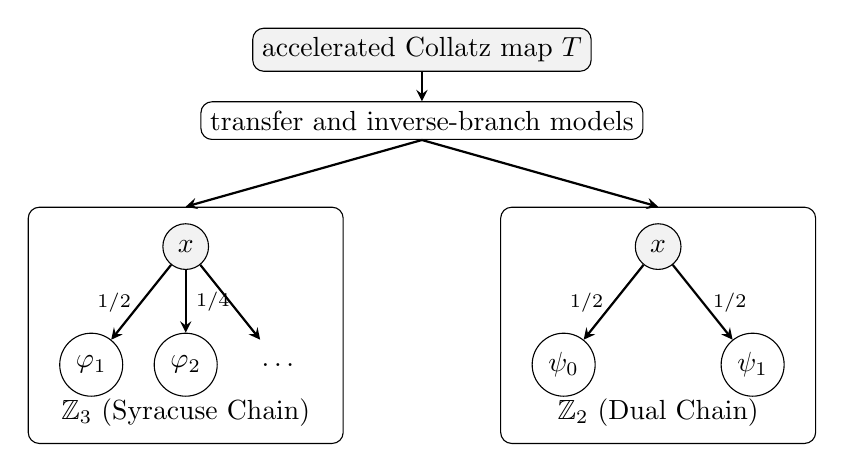
\begin{tikzpicture}[
        scale=1,
        every node/.style={transform shape}
        ]
        \node[draw, rounded corners, fill=gray!10, minimum width=3.5cm] (collatz) at (3, 3.5) {accelerated Collatz map $T$};
        \node[draw, rounded corners, minimum width=3.5cm] (transfer) at (3, 2.6) {transfer and inverse-branch models};
        \draw[->, >=stealth, thick] (collatz) -- (transfer);

        % Z3 chain
        \node[draw, rounded corners, minimum width=4cm, minimum height=3cm] (z3) at (0,0) {};
        \node[above=0.1cm of z3.south] {$\Z_3$ (Syracuse Chain)};
        
        \node[circle, draw, fill=gray!10] (x3) at (0, 1) {$x$};
        \node[circle, draw, minimum size=0.8cm, inner sep=1pt] (y3a) at (-1.2, -0.5) {$\varphi_1$};
        \node[circle, draw, minimum size=0.8cm, inner sep=1pt] (y3b) at (0, -0.5) {$\varphi_2$};
        \node[circle, draw, minimum size=0.8cm, inner sep=1pt, draw=none] (y3c) at (1.2, -0.5) {$\dots$};
        
        \draw[->, >=stealth, thick] (x3) -- node[left, font=\scriptsize] {$1/2$} (y3a);
        \draw[->, >=stealth, thick] (x3) -- node[right, font=\scriptsize] {$1/4$} (y3b);
        \draw[->, >=stealth, thick] (x3) -- (y3c);
        
        % Z2 chain
        \node[draw, rounded corners, minimum width=4cm, minimum height=3cm] (z2) at (6,0) {};
        \node[above=0.1cm of z2.south] {$\Z_2$ (Dual Chain)};
        
        \node[circle, draw, fill=gray!10] (x2) at (6, 1) {$x$};
        \node[circle, draw, minimum size=0.8cm, inner sep=1pt] (y2a) at (4.8, -0.5) {$\psi_0$};
        \node[circle, draw, minimum size=0.8cm, inner sep=1pt] (y2b) at (7.2, -0.5) {$\psi_1$};
        
        \draw[->, >=stealth, thick] (x2) -- node[left, font=\scriptsize] {$1/2$} (y2a);
        \draw[->, >=stealth, thick] (x2) -- node[right, font=\scriptsize] {$1/2$} (y2b);

        \draw[->, >=stealth, thick] (transfer.south) -- (z3.north);
        \draw[->, >=stealth, thick] (transfer.south) -- (z2.north);
    \end{tikzpicture}
    \caption{Overview of the transfer models associated with the accelerated Collatz map. The Syracuse chain on $\Z_3$ (left) uses infinitely many branches $\varphi_a(x) = (3x+1)2^{-a}$ with geometric probabilities, encoding the powers of $2$ removed after an odd step. The dual inverse-branch chain on $\Z_2$ (right) uses $\psi_0(x) = 2x$ and $\psi_1(x) = \frac{2x-1}{3}$ with equal probabilities.}
    \label{fig:transfer_operators}
\end{figure}

\begin{lemma}[Geometric law of the $2$-adic valuation]\label{lem:geometric}
For $a \ge 1$, the set of odd integers $n$ with $\nutwo(3n+1) = a$ is exactly one residue class modulo $2^{a+1}$, consisting of odd residues. Consequently, if $n$ is drawn uniformly from the odd residues modulo $2^k$, then $\Pr[\nutwo(3n+1) = a] = 2^{-a}$ for every $1 \le a \le k-1$.
\end{lemma}

\begin{proof}
For odd $n$, $3n+1$ is even, so $\nutwo(3n+1) \ge 1$. For $a \ge 1$, $\nutwo(3n+1) = a$ iff $3n+1 \equiv 2^a \pmod{2^{a+1}}$, i.e.\ $n \equiv 3^{-1}(2^a - 1) \pmod{2^{a+1}}$, a single residue class modulo $2^{a+1}$ ($3$ is invertible modulo any power of $2$); it consists of odd numbers because $2^a - 1$ and $3^{-1}$ are both odd. Among the $2^{k-1}$ odd residues modulo $2^k$, this class contains exactly $2^{k-a-1}$ of them, giving probability $2^{k-a-1}/2^{k-1} = 2^{-a}$.
\end{proof}

\begin{definition}[Syracuse chain on $\Zthree$]\label{def:syracusechain}
Since $2$ is a unit in $\Zthree$, the maps
\[
\varphi_a(x) \;=\; (3x+1)\,2^{-a}, \qquad a \ge 1,
\]
are well defined on $\Zthree$. The \emph{Syracuse chain} is the Markov kernel on $\Zthree$
\[
P(x,\cdot) \;=\; \sum_{a \ge 1} 2^{-a}\, \delta_{\varphi_a(x)} .
\]
By Lemma~\ref{lem:geometric} this is the transfer model of the Syracuse map under which Tao constructs the Syracuse random variables \cite{tao2022}.
\end{definition}

\begin{theorem}[Contraction on $\Zthree$]\label{thm:z3}
\textbf{Assumptions:} Let $P$ be the Syracuse Markov chain on $\Zthree$ generated by the branches $\varphi_a(x) = (3x+1)2^{-a}$ with probabilities $2^{-a}$. Let $P_k$ denote its projection onto $\Z/3^k\Z$.

\textbf{Conclusion:} Each branch $\varphi_a$ scales the $3$-adic metric exactly by $1/3$, meaning $|\varphi_a(x) - \varphi_a(y)|_3 = \tfrac13|x-y|_3$. Consequently, the Dobrushin--Wasserstein coefficient $\tau(P)$ is at most $1/3$, and the same bound holds for every projection $P_k$. In particular, $P$ has a unique invariant measure $\pi$ on $\Zthree$, distributions converge geometrically in $\dW$ at rate $3^{-n}$, and $\operatorname{spec}(U|_{\Lip(\Zthree)}) \subseteq \{1\} \cup \{z : |z| \le 1/3\}$.
\end{theorem}

\textbf{Interpretation:}
This result ensures that the probabilistic transfer model of the odd Collatz steps contracts geometrically in the Wasserstein metric. Although it does not prove pointwise convergence of individual trajectories (as $\Z_+$ is Haar-null in $\Z_3$), it guarantees that random distributions over trajectories converge uniquely and rapidly to the Syracuse measure, ruling out multiple competing stationary distributions.

\begin{proof}
For the branch identity: $\varphi_a(x) - \varphi_a(y) = 3(x-y)2^{-a}$, and $|3|_3 = \tfrac13$, $|2^{-a}|_3 = 1$, so $|\varphi_a(x)-\varphi_a(y)|_3 = \tfrac13 |x-y|_3$ exactly.

For $\tau(P) \le 1/3$, couple $P(x,\cdot)$ and $P(y,\cdot)$ \emph{synchronously}: draw a single $a$ with $\Pr[a] = 2^{-a}$ and move both points along the same branch $\varphi_a$. This is a coupling of the two transition laws, of cost
\[
\sum_{a\ge1} 2^{-a}\, |\varphi_a(x) - \varphi_a(y)|_3 \;=\; \tfrac13 |x-y|_3 ,
\]
so $\dW(P(x,\cdot), P(y,\cdot)) \le \tfrac13 d(x,y)$ for all $x \ne y$.

For the projections: on $\Z/3^k\Z$ put $d_k(r,s) = 3^{-v_3(r-s)}$ for $r \neq s$ (well defined since $v_3(r-s) \le k-1$). The projected kernel $P_k(r,\cdot)$ is the pushforward of $P(x,\cdot)$ under reduction modulo $3^k$, for any lift $x$ of $r$ (the reduction of $\varphi_a(x)$ modulo $3^k$ depends only on $x \bmod 3^k$, indeed only on $x \bmod 3^{k-1}$). The same synchronous coupling projects to a coupling of $P_k(r,\cdot)$ and $P_k(s,\cdot)$; each coupled pair $(\varphi_a(x) \bmod 3^k,\ \varphi_a(y) \bmod 3^k)$ either coincides (cost $0$, which happens when $v_3(x-y) = k-1$) or lies at distance $3^{-v_3(x-y)-1} = \tfrac13 d_k(r,s)$. Hence $\dW(P_k(r,\cdot), P_k(s,\cdot)) \le \tfrac13 d_k(r,s)$ and $\tau(P_k) \le \tfrac13$.

The remaining assertions follow from Lemma~\ref{lem:dobrushin} with $\tau = 1/3$.
\end{proof}

\begin{proposition}[Monotonicity and periodicity of the finite coefficients]\label{prop:taumonotone}
For every $k \ge 2$, the kernel $P_k$ is the exact pushforward of $P_{k+1}$ under reduction modulo $3^k$: for every state $r$ of $P_k$ and every lift $s$ of $r$ to a state of $P_{k+1}$, pushing $P_{k+1}(s,\cdot)$ forward under $x \mapsto x \bmod 3^k$ reproduces $P_k(r,\cdot)$ exactly. Consequently $\tau(P_k) \le \tau(P_{k+1})$ for every $k \ge 2$, and $\tau(P_k) \le \tau(P)$ for every $k$: the sequence $(\tau(P_k))_{k \ge 2}$ is nondecreasing and, by Theorem~\ref{thm:z3}, bounded above by $1/3$, hence convergent to some limit $L \in (0,1/3]$ with $\tau(P) \ge L$.

Moreover, $P_k(r,\cdot)$ depends only on $r \bmod 3^{k-1}$ (the target residue $3r+1 \bmod 3^k$ depends only on $r \bmod 3^{k-1}$), so any pair $r \ne s$ at the finest possible resolution $v_3(r-s) = k-1$ satisfies $P_k(r,\cdot) = P_k(s,\cdot)$ exactly and contributes ratio $0$ to $\tau(P_k)$. This is why the maximizing pair of $\tau(P_k)$, computed exactly in Section~\ref{sec:results-wasserstein}, is never found at the finest resolution but one level coarser.
\end{proposition}

\begin{proof}
Both $P_k(r,\cdot)$ and $P_{k+1}(s,\cdot)$ are built from the same target $3s+1 \bmod 3^{k+1}$, whose reduction modulo $3^k$ equals $3(s \bmod 3^k) + 1 = 3r+1 \bmod 3^k$; the branch weights $2^{-a}$, summed over $a$ periodic with period $\mathrm{ord}_{k+1} = 3 \cdot \mathrm{ord}_k$ (since $2$ is a primitive root modulo $3^{k+1}$), regroup exactly into the level-$k$ weights after reducing targets modulo $3^k$. Hence the pushforward of $P_{k+1}(s,\cdot)$ modulo $3^k$ reproduces $P_k(r,\cdot)$ term by term. Since reduction modulo $3^k$ is $1$-Lipschitz for the $3$-adic metric, pushforward under it cannot increase the Wasserstein cost of any coupling; applying this to the optimal coupling of $P_{k+1}(x,\cdot)$ and $P_{k+1}(y,\cdot)$ for canonical lifts $x,y$ of $r,s$ gives $\dW(P_k(r,\cdot),P_k(s,\cdot)) \le \dW(P_{k+1}(x,\cdot),P_{k+1}(y,\cdot))$; since $d_k(r,s) = d_{k+1}(x,y)$ for canonical lifts, taking the supremum over pairs gives $\tau(P_k) \le \tau(P_{k+1})$. The same argument against the infinite kernel $P$ (using the pushforward identity from the proof of Theorem~\ref{thm:z3}) gives $\tau(P_k) \le \tau(P)$ for every $k$.

For the periodicity claim: $3(r + 3^{k-1}) = 3r + 3^k \equiv 3r \pmod{3^k}$, so $r$ and $r + 3^{k-1}$ (and $r + 2\cdot 3^{k-1}$) share the same target residue at every branch $a$, hence the same full transition law.
\end{proof}

We now determine the finite-level coefficients exactly and show that the bound $1/3$ of Theorem~\ref{thm:z3} is sharp. Throughout, $c = c_k = 2\cdot 3^{k-2}$ denotes one third of the multiplicative order $\operatorname{ord}(2 \bmod 3^k) = 2 \cdot 3^{k-1} = 3c$ ($2$ is a primitive root modulo $3^k$), and $q = q_k = 2^{-c_k}$. Recall from the proof of Theorem~\ref{thm:z3} that the row of $P_k$ at an arbitrary state $r \in \Z/3^k\Z$ is obtained by grouping the branch weights $2^{-a}$ along residues of $a$ modulo $3c$:
\begin{equation}\label{eq:rowform}
P_k(r,\cdot) \;=\; \sum_{a=1}^{3c} w_a\, \delta_{t_a(r)}, \quad t_a(r) = (3r+1)\,2^{-a} \bmod 3^k, \quad w_a = \frac{2^{-a}}{1 - 2^{-3c}} ,
\end{equation}
with $3c$ pairwise distinct atoms: $3r+1 \equiv 1 \pmod 3$ is a unit of $\Z/3^k\Z$ for \emph{every} $r$, and the units $2^{-a}$, $1 \le a \le 3c$, are pairwise distinct. (The chain visits only states $3 \nmid r$, on which the exact computations of Section~\ref{sec:results-wasserstein} run; formula \eqref{eq:rowform} and everything below hold verbatim for all $r \in \Z/3^k\Z$, which is the generality needed to discuss the supremum over $\Zthree$.)

\begin{lemma}[Collision structure at valuation $k-2$]\label{lem:collision}
Let $k \ge 2$ and let $r, s \in \Z/3^k\Z$ satisfy $v_3(r-s) = k-2$, say $s = r + 3^{k-2}u$ with $3 \nmid u$. Then:
\begin{enumerate}
\item $2^{c} \equiv 1 + 3^{k-1} \pmod{3^k}$ and $2^{2c} \equiv 1 + 2\cdot 3^{k-1} \pmod{3^k}$; consequently, for $m \in \Z$, $v_3(2^m - 1) = k - 1$ holds precisely when $m \equiv c$ or $m \equiv 2c \pmod{3c}$.
\item The pushforwards of $P_k(r,\cdot)$ and $P_k(s,\cdot)$ under reduction modulo $3^{k-1}$ coincide exactly, and the total-variation distance of the two rows at level $k$ is
\[
\tfrac12 \sum_{z \bmod 3^k} \bigl| P_k(r,z) - P_k(s,z) \bigr| \;=\; \frac{(1-q)(1-q^2)}{1-q^3} \;=\; \frac{1-q^2}{1+q+q^2} .
\]
\item Consequently, by Lemma~\ref{lem:w1formula},
\[
\dW\bigl(P_k(r,\cdot),\, P_k(s,\cdot)\bigr) \;=\; 3^{-(k-1)}\, \frac{1-q^2}{1+q+q^2},
\]
independently of $r$ and $u$: every pair on the sphere $v_3(r-s) = k-2$ realizes the same Wasserstein distance, hence the same ratio $\dW/d_k(r,s) = \tfrac13 (1-q^2)/(1+q+q^2)$.
\end{enumerate}
\end{lemma}

\begin{proof}
(1) Induction on $k$. For $k = 2$: $2^{c_2} = 2^2 = 1 + 3$. Assume $2^{c_k} = 1 + 3^{k-1}(1 + 3t)$ for some $t \in \Z$. Since $c_{k+1} = 3c_k$, cubing gives
\begin{align*}
2^{c_{k+1}} = \bigl(1 + 3^{k-1}(1+3t)\bigr)^3
&= 1 + 3\cdot 3^{k-1}(1+3t) + 3\cdot 3^{2(k-1)}(1+3t)^2 \\
&\qquad + 3^{3(k-1)}(1+3t)^3
\;\equiv\; 1 + 3^{k} \pmod{3^{k+1}},
\end{align*}
because $2k - 1 \ge k + 1$ and $3k - 3 \ge k + 1$ for $k \ge 2$. Squaring $2^c \equiv 1 + 3^{k-1}$ gives $2^{2c} \equiv 1 + 2\cdot 3^{k-1} + 3^{2k-2} \equiv 1 + 2 \cdot 3^{k-1} \pmod{3^k}$ (as $2k-2 \ge k$). For the valuation claim: $v_3(2^m-1) \ge k-1$ means $2^m \equiv 1 \pmod{3^{k-1}}$, which holds iff $\operatorname{ord}(2 \bmod 3^{k-1}) = c$ divides $m$; and $v_3(2^m - 1) \ge k$ iff $\operatorname{ord}(2 \bmod 3^{k}) = 3c$ divides $m$. Hence $v_3(2^m-1) = k-1$ iff $m \equiv c, 2c \pmod{3c}$, with unit parts $(2^m-1)/3^{k-1} \equiv 1$ resp.\ $2 \pmod 3$ by the two congruences just proved.

(2) Write $t_a = t_a(r)$ and $t'_a = t_a(s)$ for the atoms \eqref{eq:rowform} of the two rows. Since $3s + 1 = 3r + 1 + 3^{k-1}u$ and $2^{-a} \equiv (-1)^a \pmod 3$,
\[
t'_a \;=\; t_a + 3^{k-1} u\, 2^{-a} \;\equiv\; t_a + (-1)^a u\, 3^{k-1} \pmod{3^k}.
\]
Reduction modulo $3^{k-1}$ kills the shift, so the two rows have identical pushforwards at level $k-1$ (hence at every coarser level), proving the first claim of (2).

At level $k$, the two rows are supported on $3c$ atoms each, and the total variation distance equals $1 - \sum_z \min\{P_k(r,z), P_k(s,z)\}$, where the overlap sum runs over coincidences $t_b = t'_a$. By the display above, $t_b = t'_a$ amounts to $(3r+1)(2^{-b} - 2^{-a}) \equiv (-1)^a u\, 3^{k-1} \pmod{3^k}$, i.e.
\[
-(3r+1)\, 2^{-b} \bigl(2^{\,b-a} - 1\bigr) \equiv (-1)^a u\, 3^{k-1} \pmod{3^k}.
\]
The right-hand side has $3$-adic valuation exactly $k-1$, so by (1) a coincidence requires $m := b - a \equiv c$ or $2c \pmod{3c}$. Two residues of valuation exactly $k-1$ agree modulo $3^k$ iff their quotients by $3^{k-1}$ agree modulo $3$; using $3r+1 \equiv 1$, $2^{-b} \equiv (-1)^b \pmod 3$, $(-1)^b = (-1)^a$ (both admissible $m$ are even), and the unit parts from (1), the coincidence condition reduces to
\[
-\,e_m \equiv u \pmod 3, \qquad e_m := \frac{2^m - 1 \bmod 3^k}{3^{k-1}} \equiv \begin{cases} 1, & m \equiv c, \\ 2, & m \equiv 2c \end{cases} \pmod 3 .
\]
Hence exactly one shift class $m^* \in \{c, 2c\}$ occurs: $m^* = 2c$ if $u \equiv 1 \pmod 3$, and $m^* = c$ if $u \equiv 2 \pmod 3$. The coincidences are therefore exactly the pairs $(a, b)$ with $b \equiv a + m^* \pmod{3c}$: a bijection between the atom sets. Representing indices in $\{1, \dots, 3c\}$, the matched weight is $\min\{w_a, w_{\sigma(a)}\} = w_{\max\{a, \sigma(a)\}}$ with $\sigma(a) = a + m^*$ if $a \le 3c - m^*$ and $\sigma(a) = a + m^* - 3c$ otherwise, so
\begin{align*}
(1 - 2^{-3c}) \sum_{a=1}^{3c} \min\{w_a, w_{\sigma(a)}\}
&= \sum_{a=1}^{3c-m^*} 2^{-(a+m^*)} + \!\!\sum_{a = 3c-m^*+1}^{3c}\!\! 2^{-a} \\
&= 2^{-m^*} + 2^{-(3c - m^*)} - 2\cdot 2^{-3c} .
\end{align*}
For both $m^* \in \{c, 2c\}$ the right-hand side equals $q + q^2 - 2q^3$, so the overlap is $(q + q^2 - 2q^3)/(1 - q^3)$ regardless of $u$, and the total variation distance is
\[
1 - \frac{q + q^2 - 2q^3}{1 - q^3} \;=\; \frac{1 - q - q^2 + q^3}{1 - q^3} \;=\; \frac{(1-q)(1-q^2)}{1-q^3} .
\]

(3) In Lemma~\ref{lem:w1formula} (with $p = 3$, $\ell$ ranging up to $k$), the first claim of (2) gives $m_\ell = 0$ for every $\ell \le k-1$, and $m_k$ is the total variation distance just computed; the formula collapses to $\dW = 3^{-(k-1)} m_k$. Dividing by $d_k(r,s) = 3^{-(k-2)}$ gives the stated ratio.
\end{proof}

\begin{theorem}[Closed form of $\tau(P_k)$; the $1/3$ bound is sharp and not attained]\label{thm:tausharp}
Let $q_k = 2^{-2\cdot 3^{k-2}}$ and set
\[
\rho_k \;=\; \frac13 \cdot \frac{1 - q_k^2}{1 + q_k + q_k^2} .
\]
\begin{enumerate}
\item \textbf{(Closed form.)} For every $k \ge 2$, $\tau(P_k) = \rho_k$, and the maximum defining $\tau(P_k)$ is attained exactly on the pairs with $v_3(r - s) = k-2$, each of which realizes it --- e.g.\ the explicit family $(1,\, 1 + 3^{k-2})$. In particular $\tau_2 = \tfrac{5}{21}$, $\tau_3 = \tfrac{455}{1387}$, $\tau_4 = \tfrac{7635497415}{22906579627}$.
\item \textbf{(Doubly exponential collapse.)} The sequence $\tau(P_k)$ is strictly increasing and
\[
0 \;<\; \frac13 - \tau(P_k) \;=\; \frac{q_k (1 + 2 q_k)}{3\,(1 + q_k + q_k^2)} \;<\; q_k = 2^{-2\cdot 3^{k-2}} .
\]
\item \textbf{(Sharpness.)} $\tau(P) = \lim_k \tau(P_k) = 1/3$: the synchronous-coupling bound of Theorem~\ref{thm:z3} is sharp. Equivalently, by Kantorovich--Rubinstein duality, the norm of the Koopman operator $U$ on $\Lip(\Zthree)$ modulo constants is exactly $1/3$.
\item \textbf{(Non-attainment.)} The supremum defining $\tau(P)$ is attained by no pair: for all $x \ne y$ in $\Zthree$ with $v = v_3(x-y)$,
\[
\frac{\dW\bigl(P(x,\cdot), P(y,\cdot)\bigr)}{d(x,y)} \;\le\; \frac13 - \frac29\,\omega_v \;<\; \frac13,
\qquad
\omega_v := \frac{q' + q'^2 - 2q'^3}{1 - q'^3},
\]
where $q' = 2^{-2\cdot 3^{v}}$. The pairs $(1,\, 1 + 3^{k-2})$, $k \to \infty$, form an explicit maximizing family.
\end{enumerate}
\end{theorem}

\begin{proof}
(1) By Lemma~\ref{lem:collision}(3), every pair on the sphere $v_3(r-s) = k-2$ has ratio exactly $\rho_k$, so $\tau(P_k) \ge \rho_k$; it remains to show no other pair exceeds it. Pairs with $v_3(r-s) = k-1$ have identical rows (Proposition~\ref{prop:taumonotone}) and contribute ratio $0$. Let now $v := v_3(r - s) \le k-3$ (which requires $k \ge 3$). In Lemma~\ref{lem:w1formula}, the discrepancy $m_\ell$ of the pair $(P_k(r,\cdot), P_k(s,\cdot))$ at level $\ell$ equals the level-$\ell$ discrepancy of the reduced pair under the projected kernel $P_\ell$, by the projectivity of Proposition~\ref{prop:taumonotone}. Hence: $m_\ell = 0$ for $\ell \le v + 1$ (the rows of $P_\ell$ depend on the state modulo $3^{\ell-1}$ and $r \equiv s \bmod 3^{v}$); $m_{v+2} = 1 - \omega_v$ by Lemma~\ref{lem:collision}(2) applied at level $v+2$, where the reduced pair sits on the sphere of valuation $(v+2)-2$; and $m_\ell \le 1$ for $\ell > v+2$. Therefore
\[
\dW \;\le\; \bigl(3^{-(v+1)} - 3^{-(v+2)}\bigr)(1 - \omega_v) \;+\; 3^{-(v+2)}
\qquad\Longrightarrow\qquad
\frac{\dW}{3^{-v}} \;\le\; \frac13 - \frac29\, \omega_v .
\]
It remains to check $\tfrac29 \omega_v > \tfrac13 - \rho_k$ for all $0 \le v \le k-3$. Since $q' \le \tfrac14$ and $(1+2q')/(1-q'^3) \ge 1$, we have $\omega_v = q'(1+2q')(1-q')/(1-q'^3) \ge q'(1 - q') \ge \tfrac34 q'$; and $q' = 2^{-2\cdot 3^v} \ge 2^{-2 \cdot 3^{k-3}} = q_k^{1/3}$, so $\tfrac29 \omega_v \ge \tfrac16 q_k^{1/3}$. On the other side, $\tfrac13 - \rho_k \le q_k$ by (2). Finally $\tfrac16 q_k^{1/3} > q_k$ iff $q_k^{2/3} < \tfrac16$, which holds because $q_k \le 2^{-6}$ for $k \ge 3$. Hence $\tau(P_k) = \rho_k$, attained exactly on the sphere of valuation $k-2$.

(2) A direct computation gives $\tfrac13 - \rho_k = \tfrac13 (q_k + 2q_k^2)/(1 + q_k + q_k^2) = q_k(1+2q_k)/(3(1+q_k+q_k^2))$, which is positive and less than $q_k$ (as $1 + 2q < 3(1+q+q^2)$). The map $q \mapsto \tfrac13(1-q^2)/(1+q+q^2)$ has derivative of sign $-(1 + 4q + q^2) < 0$, so it is strictly decreasing; $q_k$ is strictly decreasing in $k$, hence $\rho_k$ is strictly increasing.

(3) By Proposition~\ref{prop:taumonotone} and Theorem~\ref{thm:z3}, $\rho_k = \tau(P_k) \le \tau(P) \le \tfrac13$ for every $k$, and $\rho_k \to \tfrac13$ by (2); hence $\tau(P) = \lim_k \tau(P_k) = \tfrac13$. For the operator norm: duality gives $\sup_{f} \Lip(Uf)/\Lip(f) = \tau(P)$, since $|Uf(x) - Uf(y)| \le \Lip(f)\, \dW(P(x,\cdot),P(y,\cdot))$ with equality approached by Kantorovich potentials of the pair $(P(x,\cdot), P(y,\cdot))$.

(4) We first record an approximation identity: for Borel probability measures $\mu, \nu$ on $\Zthree$,
\[
\dW(\mu, \nu) \;=\; \lim_{j \to \infty} \dW\bigl(\pi_{j\#}\mu,\, \pi_{j\#}\nu\bigr),
\]
where $\pi_j : \Zthree \to \Z/3^j\Z$ is reduction and the right-hand sequence is nondecreasing. Indeed, $\pi_j$ is $1$-Lipschitz onto $(\Z/3^j\Z, d_j)$, so pushforward does not increase $\dW$, and $\pi_j$ factors through $\pi_{j+1}$ via a further $1$-Lipschitz reduction, giving monotonicity. Conversely, let $s_j : \Z/3^j\Z \to \Zthree$ send each residue to its integer representative in $[0, 3^j)$. Then $\pi_j \circ s_j = \mathrm{id}$, $|s_j(r) - s_j(r')|_3 = d_j(r, r')$ for $r \ne r'$ (an isometric embedding, so pushforward under $s_j$ preserves $\dW$ exactly), and $|x - s_j(\pi_j x)|_3 \le 3^{-j}$ for every $x$, so the deterministic coupling along $x \mapsto s_j(\pi_j x)$ gives $\dW(\mu, s_{j\#}\pi_{j\#}\mu) \le 3^{-j}$. The triangle inequality then yields $\dW(\mu,\nu) \le \dW(\pi_{j\#}\mu, \pi_{j\#}\nu) + 2\cdot 3^{-j}$, and the identity follows.

Now let $x \ne y$ in $\Zthree$, $v = v_3(x - y)$. By the pushforward identity (proof of Theorem~\ref{thm:z3}), $\pi_{j\#} P(x,\cdot) = P_j(\pi_j x, \cdot)$. For every $j \ge v + 3$, the reduced pair $(\pi_j x, \pi_j y)$ has valuation $v \le j - 3$, so the level-$j$ bound established in the proof of (1) gives
\[
\dW\bigl(P_j(\pi_j x,\cdot),\, P_j(\pi_j y,\cdot)\bigr) \;\le\; \Bigl(\frac13 - \frac29\,\omega_v\Bigr)\, 3^{-v} .
\]
Letting $j \to \infty$ and using $d(x,y) = 3^{-v}$ proves the displayed bound; $\omega_v > 0$ makes it strictly less than $\tfrac13$, so no pair attains the supremum. Finally, for the pair $x_k = 1$, $y_k = 1 + 3^{k-2}$ (as elements of $\Zthree$), monotonicity of the finite-level approximants gives
\[
\frac{\dW\bigl(P(x_k,\cdot), P(y_k,\cdot)\bigr)}{d(x_k,y_k)} \;\ge\; \frac{\dW\bigl(P_k(\pi_k x_k,\cdot), P_k(\pi_k y_k,\cdot)\bigr)}{3^{-(k-2)}} \;=\; \rho_k \;\xrightarrow[k\to\infty]{}\; \frac13 ,
\]
so this family is maximizing.
\end{proof}

\begin{remark}\label{rem:tauk}
Theorem~\ref{thm:tausharp} closes the question left open in an earlier version of this work: the finite-level coefficients, previously known only as a proved nondecreasing sequence with exact values at $k \le 5$, are now given in closed form, and the limit is identified with $\tau(P) = 1/3$ exactly. Two structural features are worth noting. First, the extremal geometry is a \emph{sphere, not a pair}: at each level every pair at $3$-adic distance $3^{-(k-2)}$ --- one step coarser than the finest resolution, where rows collapse --- realizes the maximum, and on $\Zthree$ itself the supremum is attained by no pair at all. Second, the collapse of the gap $1/3 - \tau_k < 2^{-2\cdot 3^{k-2}}$ is doubly exponential in $k$ because the overlap of the two extremal rows is governed by the tail $2^{-\operatorname{ord}(2 \bmod 3^{k-1})}$ of the geometric branch weights; this explains the numerically observed gap $1/3 - \tau_5 \approx 1.85\times 10^{-17}$, which is exactly $q_5(1+2q_5)/(3(1+q_5+q_5^2))$ with $q_5 = 2^{-54}$. The exact brute-force values of Section~\ref{sec:results-wasserstein} now serve as independent finite-level certificates of the closed form. We stress the scope of Remark~\ref{rem:scope}: sharpness refines the measure-theoretic contraction picture; it says nothing new about pointwise orbits on $\Z_+$.
\end{remark}

We now turn to the dual chain on $\Ztwo$. The accelerated map $T$ extends continuously to $\Ztwo$ and preserves Haar measure; it is conjugate to the one-sided Bernoulli shift \cite{terras1976,lagarias1985,bernsteinlagarias1996}, an instance of the general theory of measure-preserving and Bernoulli transformations on the $p$-adic integers \cite{kingsberyetal2009,kingsberyetal2011}. Its transfer (backward) chain is driven by the two inverse branches of $T$ on $\Ztwo$:
\[
\psi_0(x) = 2x \ (\text{even step}), \quad
\psi_1(x) = \tfrac{2x-1}{3} \ (\text{odd step}),
\]
both well defined on $\Ztwo$ since $3$ is a unit in $\Ztwo$.

\begin{theorem}[Contraction and finite-time Haar averaging on $\Ztwo$]\label{thm:z2}
\textbf{Assumptions:} Let $Q$ be the Markov kernel on $\Ztwo$ given by $Q(x,\cdot) = \tfrac12 \delta_{\psi_0(x)} + \tfrac12 \delta_{\psi_1(x)}$, with Koopman operator $Lf(x) = \tfrac12 f(2x) + \tfrac12 f\bigl(\tfrac{2x-1}{3}\bigr)$.

\textbf{Conclusion:} The Dobrushin--Wasserstein coefficient $\tau(Q)$ is exactly $1/2$. Haar measure on $\Ztwo$ is the unique invariant measure of $Q$. Furthermore, if $f : \Ztwo \to \R$ depends only on $x \bmod 2^k$ (a level-$k$ cylinder function), then $L^k f$ is identically equal to the exact Haar average $2^{-k} \sum_{r \bmod 2^k} f(r)$.
\end{theorem}

\textbf{Interpretation:}
On the $2$-adic integers, the backward map acts essentially like a fair coin flip. The Wasserstein metric captures this perfectly: any observable that only depends on the first $k$ digits of the state is completely forgotten (averaged out) after exactly $k$ steps. This provides a clean, dimension-free geometric explanation for why parity vectors perfectly equidistribute.

\begin{proof}
Both branches scale the metric by exactly $1/2$: $|\psi_0(x)-\psi_0(y)|_2 = |2|_2 |x-y|_2 = \tfrac12|x-y|_2$, and $|\psi_1(x)-\psi_1(y)|_2 = |2(x-y)/3|_2 = \tfrac12 |x-y|_2$ since $|3|_2 = 1$.

(1) The synchronous coupling (same branch on both points) gives cost exactly $\tfrac12|x-y|_2$, so $\dW \le \tfrac12 |x-y|_2$. For the reverse inequality, note the cross distances are maximal: $\psi_0(x) - \psi_1(y) = 2x - \tfrac{2y-1}{3} = \tfrac{6x - 2y + 1}{3}$ has odd numerator and unit denominator, so $|\psi_0(x)-\psi_1(y)|_2 = 1 \ge \tfrac12|x-y|_2$ (as $|x-y|_2 \le 1$), and symmetrically. Thus \emph{every} coupling of the two two-point laws transports each unit of mass a distance at least $\tfrac12|x-y|_2$, whence $\dW \ge \tfrac12|x-y|_2$.

(2) Uniqueness follows from (1) and Lemma~\ref{lem:dobrushin}. For invariance of Haar measure $\lambda$: $\psi_0$ is a homeomorphism of $\Ztwo$ onto $2\Ztwo$ (the even $2$-adics) with $(\psi_0)_*\lambda = 2\,\lambda|_{2\Ztwo}$ (it scales Haar mass by $|2|_2 = \tfrac12$ onto a set of measure $\tfrac12$, uniformly), and $\psi_1$ is a homeomorphism onto $1 + 2\Ztwo$ (the odd $2$-adics: $2x-1$ is odd and division by the unit $3$ preserves $2$-adic parity) with $(\psi_1)_*\lambda = 2\,\lambda|_{1+2\Ztwo}$. Hence
\[
\lambda Q \;=\; \tfrac12 (\psi_0)_*\lambda + \tfrac12 (\psi_1)_*\lambda \;=\; \lambda|_{2\Ztwo} + \lambda|_{1+2\Ztwo} \;=\; \lambda .
\]

(3) For a word $u = (u_1,\dots,u_k) \in \{0,1\}^k$ write $\psi_u = \psi_{u_1} \circ \cdots \circ \psi_{u_k}$. Then
\[
L^k f(x) \;=\; 2^{-k} \sum_{u \in \{0,1\}^k} f\bigl(\psi_u(x)\bigr).
\]
Since each branch scales the metric by $\tfrac12$, $|\psi_u(x) - \psi_u(y)|_2 = 2^{-k}|x-y|_2 \le 2^{-k}$, so $\psi_u(x) \bmod 2^k$ does not depend on $x$; as $f$ is a level-$k$ cylinder function, each summand is a constant $c_u$. We claim the map $u \mapsto \psi_u(x) \bmod 2^k$ is a bijection onto $\Z/2^k\Z$: by induction on $k$, the images of $\psi_0$ and $\psi_1$ lie in the (disjoint) even and odd classes respectively, and within each class, $\psi_i$ composed with the $2^{k-1}$ maps $\psi_{u'}$ ($u' \in \{0,1\}^{k-1}$) yields $2^{k-1}$ points that are pairwise distinct modulo $2^k$, because $\psi_i$ maps points distinct modulo $2^{k-1}$ to points distinct modulo $2^k$ (exact $\tfrac12$-scaling of the metric). Hence $\{c_u\}_u$ enumerates $\{f(r) : r \bmod 2^k\}$ exactly once and $L^k f \equiv 2^{-k}\sum_{r} f(r) = \int f \,\mathrm{d}\lambda$.
\end{proof}

\begin{remark}\label{rem:duality}
Theorem~\ref{thm:z2}(3) is the functional-analytic reading of Terras's conjugacy with the Bernoulli shift \cite{terras1976}: the backward chain forgets the level-$k$ observable in exactly $k$ steps, i.e.\ mixing is not merely geometric but \emph{finite-time} on cylinder observables. It is also the exact analogue of the finite-level rank collapse of the Syracuse chain (Proposition~\ref{prop:rankcollapse}).
\end{remark}

\begin{remark}[Scope of the contraction theorems]\label{rem:scope}
Theorems~\ref{thm:z3} and \ref{thm:z2} operate on spaces of \emph{global densities} over the compact rings $\Zthree$, $\Ztwo$. The set $\Z_+$ where the conjecture lives is Haar-null in both. Contraction of distributions in $\dW$ therefore does not, by itself, constrain individual orbits: in $\ell^1(\Z_+)$, every finite section of the pushforward operator we tested is nilpotent (spectrum $\{0\}$), and no elementary weight $n^\theta$ yields uniform contraction --- the obstruction being, again, the residue classes $n \equiv -1 \bmod 2^t$ of Theorem~\ref{thm:main} (Section~\ref{sec:results-wasserstein}). We state this limitation explicitly to avoid overclaiming: the contraction theorems quantify the measure-theoretic ingredient of ``almost-all'' results in the style of \cite{terras1976,tao2022}; they do not approach the pointwise conjecture.
\end{remark}

\section{Exact algorithms}\label{sec:algorithms}

This section describes the algorithms behind the verifications of Section~\ref{sec:results} and proves the statements they rely on. Implementation details of the arithmetic are deferred to Section~\ref{sec:methodology}.

\subsection{Cycle enumeration via parity vectors}\label{sec:cycles-alg}

\begin{proposition}[Affine form and cycle equation]\label{prop:cycleform}
Fix $d$ odd and let $p = (p_0,\dots,p_{L-1}) \in \{0,1\}^L$ be the parity vector of the first $L$ accelerated steps of $n$ in the $3n+d$ system, with $k = \sum_i p_i$. Then
\[
T_d^L(n) \;=\; \frac{3^k n + b(p)}{2^L},
\]
where $b(p) = b_L$ is given by the recurrence
\[
b_0 = 0,\qquad b_{i+1} = \begin{cases} 3 b_i + d\, 2^i, & p_i = 1,\\ b_i, & p_i = 0.\end{cases}
\]
Consequently $n$ lies on a cycle of length $L$ with parity vector $p$ if and only if
\begin{equation}\label{eq:cycleeq}
n \;=\; \frac{b(p)}{2^L - 3^k},
\end{equation}
which for $L \geq 1$ has at most one solution ($2^L \neq 3^k$).
\end{proposition}

\begin{proof}
By induction on $i$: writing $k_i = p_0 + \dots + p_{i-1}$, assume $T_d^i(n) = (3^{k_i} n + b_i)/2^i$ (true for $i=0$). If $p_i = 0$, the next step halves: $T_d^{i+1}(n) = (3^{k_i} n + b_i)/2^{i+1}$ and $b_{i+1} = b_i$. If $p_i = 1$,
\[
T_d^{i+1}(n) = \frac{3\,T_d^i(n) + d}{2} = \frac{3(3^{k_i} n + b_i)/2^i + d}{2} = \frac{3^{k_i+1} n + 3b_i + d\,2^i}{2^{i+1}},
\]
matching the recurrence. The cycle condition $T_d^L(n) = n$ then reads $n(2^L - 3^k) = b(p)$.
\end{proof}

The enumeration algorithm tests \eqref{eq:cycleeq} for every parity vector: every cycle other than the fixed point $0$ contains an odd element, so it may be rotated to begin with $p_0 = 1$, and it suffices to sweep the $2^{L-1}$ vectors with $p_0 = 1$ for each $L \le L_{\max}$. For each integral solution $n$, the algorithm \emph{re-runs the actual orbit} and keeps $n$ only if its true parity vector is $p$ and $T_d^L(n) = n$ --- eliminating algebraic solutions that do not realize their parity pattern. The output is therefore the complete list of cycles of $T_d$ in $\Z$ of length at most $L_{\max}$: exact arithmetic replaces orbit simulation as the search mechanism.

\subsection{Diophantine cycle exclusion}\label{sec:exclusion-alg}

\begin{proposition}[Cycle inequality]\label{prop:exclusion}
Suppose every integer $2 \le n \le N$ converges to the trivial cycle under $T$, and let $C$ be a nontrivial cycle of $T$ in $\Z_+$ with $k$ odd elements and total length $L$ (in $T$-steps). Then all elements of $C$ exceed $N$ and
\begin{equation}\label{eq:diophantine}
0 \;<\; L - k\alpha \;\le\; k\,\varepsilon(N), \qquad \varepsilon(N) := \log_2\Bigl(1 + \frac{1}{3N}\Bigr),
\end{equation}
where $\alpha = \log_2 3$. In particular $\|k\alpha\| \le k\,\varepsilon(N)$.
\end{proposition}

\begin{proof}
If $C$ contained an element $\le N$, that element would converge to the trivial cycle, contradicting nontriviality; so every element exceeds $N$. Let $x_1, \dots, x_k$ be the odd elements of $C$ in cyclic order, and let $2^{a_i}$ be the power of two divided out between $x_i$ and $x_{i+1}$ (indices mod $k$), so $x_{i+1} = (3x_i + 1)/2^{a_i}$ and $\sum_i a_i = L$. Multiplying around the cycle,
\[
2^L \;=\; \prod_{i=1}^{k} \frac{3x_i + 1}{x_i} \;=\; \prod_{i=1}^{k} \Bigl(3 + \frac{1}{x_i}\Bigr).
\]
Taking $\log_2$: $L - k\alpha = \sum_i \log_2\bigl(1 + \tfrac{1}{3x_i}\bigr)$, which is strictly positive and, since each $x_i > N$, at most $k \log_2(1 + \tfrac{1}{3N})$. As $L$ is an integer, $\|k\alpha\| \le L - k\alpha \le k\varepsilon(N)$.
\end{proof}

The exclusion now follows from the classical theory of best rational approximation \cite[Ch.~I--II]{khinchin1964}: if $p_i/q_i$ are the convergents of the (infinite, since $\alpha$ is irrational) continued fraction of $\alpha$, then for $q_i \le k < q_{i+1}$,
\[
\|k\alpha\| \;\ge\; \|q_i\alpha\| \;>\; \frac{1}{q_i + q_{i+1}},
\]
so \eqref{eq:diophantine} forces $k > \bigl(\varepsilon(N)\,(q_i + q_{i+1})\bigr)^{-1}$ within that range. Sweeping consecutive convergent denominators yields the largest $K$ such that every $k \le K$ is impossible; then $L > K\alpha$ bounds the cycle length, and since the $L$ iterates of a cycle are distinct, also the number of its elements. This is the method of Eliahou \cite{eliahou1993} and Simons--de Weger \cite{simonsdeweger2005}; our contribution is the certification scheme (Section~\ref{sec:methodology}) making every step exact. Numerical outcomes are in Section~\ref{sec:results-exclusion}.

\subsection{The obstruction as a graph problem: Karp's algorithm}\label{sec:karp}

Fix $j \ge 1$ and let $M = 2^j$. Define a weighted digraph $G_j$ on the vertex set $\Z/M\Z$: each residue $r$ has the two successors $T(r) \bmod M$ and $T(r + M) \bmod M$ (the images of the two lifts of $r$ modulo $2M$, which determine $T$ modulo $M$), and every edge leaving $r$ carries the weight
\[
c(r) \;=\; \begin{cases} \log_2 3 - 1, & r \text{ odd},\\ -1, & r \text{ even}. \end{cases}
\]
The weight is the exact asymptotic logarithmic gain of the step on the class: for odd $n$, $\log_2\frac{T(n)}{n} = \log_2\bigl(\frac32 + \frac{1}{2n}\bigr) \downarrow \log_2 3 - 1$ as $n \to \infty$, and for even $n$ it is exactly $-1$.

\begin{proposition}[Necessary feasibility relaxation]\label{prop:karpfeas}
If a modular Lyapunov function of level $j$ existed (Definition~\ref{def:lyap}, extended to require decrease on even steps as well), then the difference constraints
\begin{equation}\label{eq:diffcon}
w(s) - w(r) \;\le\; -c(r) \qquad \text{for every edge } r \to s \text{ of } G_j
\end{equation}
would be feasible. Conversely, \eqref{eq:diffcon} is infeasible if and only if $G_j$ contains a cycle of strictly positive total weight; and the maximum cycle mean of $G_j$ equals $\log_2 3 - 1 > 0$, attained by the self-loop at the residue $-1 \bmod M$.
\end{proposition}

\begin{proof}
\emph{Necessity.} Let $r \to s$ be an edge of $G_j$ with $r$ odd, witnessed by the lift class $\{n \equiv r' \pmod {2M}\}$ (where $r' \in \{r, r+M\}$) whose members map into class $s$. For each positive $n$ in that class, the assumed decrease gives $w(s) - w(r) < -\log_2 \frac{T(n)}{n} = -\log_2\bigl(\frac32 + \frac1{2n}\bigr)$. Letting $n \to \infty$ along the class, the right side increases to $-(\log_2 3 - 1) = -c(r)$, so $w(s) - w(r) \le -c(r)$. For $r$ even the same argument gives $w(s) - w(r) \le 1 = -c(r)$ (with equality of the bound, since $\log_2\frac{T(n)}{n} = -1$ exactly).

\emph{Feasibility criterion.} If \eqref{eq:diffcon} holds and $r_0 \to r_1 \to \dots \to r_\ell = r_0$ is a cycle, summing the constraints telescopes to $0 \le -\sum_i c(r_i)$, so every cycle has total weight $\le 0$. Conversely, suppose every cycle of $G_j$ has total weight $\le 0$, i.e.\ has cost $\ge 0$ for the edge costs $b(r \to s) := -c(r)$. Adjoin a super-source $\sigma$ with a cost-$0$ edge to every vertex, and set $w(v)$ equal to the minimum cost of a walk from $\sigma$ to $v$; this is well defined because walks cannot decrease cost by traversing cycles (all cycle costs are $\ge 0$), so the minimum is attained by a simple path. By minimality, $w(s) \le w(r) + b(r \to s)$ for every edge, which is \eqref{eq:diffcon}.

\emph{Maximum mean.} Every edge weight is at most $\log_2 3 - 1$ (as $\log_2 3 - 1 > -1$), so every cycle has mean at most $\log_2 3 - 1$. The residue $r = M - 1 \equiv -1$ is odd, and its lift $2M - 1$ satisfies
\[
T(2M-1) \;=\; \frac{3(2M-1)+1}{2} \;=\; 3M - 1 \;\equiv\; -1 \pmod{M},
\]
so $G_j$ has a self-loop at $-1 \bmod M$ of weight $\log_2 3 - 1$, attaining the bound. Its mean is positive precisely because $3 > 2$.
\end{proof}

Proposition~\ref{prop:karpfeas} recasts Theorem~\ref{thm:main} as the infeasibility of \eqref{eq:diffcon} and identifies the culprit cycle a priori. Karp's algorithm \cite{karp1978} computes the maximum cycle mean of $G_j$ and an attaining cycle by dynamic programming in $O(|V||E|)$ time; running it for a range of $j$ (Section~\ref{sec:results-karp}) verifies that the \emph{unique} optimal cycle is the predicted self-loop at $-1 \bmod 2^j$ --- the computational fingerprint of the $2$-adic fixed point.

The same optimization extends to the variable-depth rules of Section~\ref{sec:stopping}. Let $S$ be a finite maximal prefix code of depth $B = \max_{p \in S}|p|$ and fix $m \ge B$, $M = 2^m$. Since $m \ge B$, the stopping word $p(r) \in S$ of a residue class $r \bmod M$ is determined by $r$ (its first $|p(r)| \le B \le m$ parities are). Define the \emph{block graph} $G_S$ on $\Z/M\Z$: for each of the $2^{|p(r)|}$ lifts $\tilde r$ of $r$ modulo $2^{m + |p(r)|}$, an edge $r \to T^{|p(r)|}(\tilde r) \bmod M$ (well defined on the lift class), with weight
\[
c(p) \;=\; a(p)\,\alpha - |p| , \qquad a(p) = \#\{\text{ones in } p\},\quad \alpha = \log_2 3,
\]
the exact asymptotic logarithmic gain of the block on the class.

\begin{proposition}[Block relaxation and exact certificate]\label{prop:blockkarp}
Let $S$, $m$, $G_S$ be as above, and let $s = \sigma_S(-1)$ (finite by Corollary~\ref{cor:koenig}).
\begin{enumerate}
\item If a variable-depth stopping-time potential for $S$ exists with modular window $w = \tilde w(n \bmod 2^m)$, then the difference constraints $\tilde w(v) - \tilde w(r) \le -c(p(r))$, one per edge $r \to v$ of $G_S$, are feasible.
\item The constraints are infeasible if and only if $G_S$ contains a cycle of strictly positive total weight; and a cycle traversing blocks with $A$ odd steps and $L$ total steps has positive weight if and only if $3^A > 2^L$ --- an exact integer comparison.
\item Every cycle of $G_S$ has per-step gain (total weight divided by total steps) at most $\alpha - 1$, with equality precisely when every block word on the cycle is all-ones; the self-loop at $-1 \bmod M$ through the word $1^s$ attains it, with total weight $s(\alpha - 1) > 0$.
\end{enumerate}
\end{proposition}

\begin{proof}
(1) Fix an edge $r \to v$ witnessed by the lift class $\{n \equiv \tilde r \pmod{2^{m+L}}\}$, $L = |p(r)|$. For each positive odd $n$ in the class, all $L$ steps of the block follow the word $p(r)$ and end at $T^L(n) \equiv v \pmod M$, so \eqref{eq:blockdescent} gives $\tilde w(v) - \tilde w(r) \le -\log_2 \bigl(T^L(n)/n\bigr)$. Along the class $n \to \infty$, each odd step contributes $\log_2(\tfrac32 + \tfrac1{2x}) \downarrow \alpha - 1$ and each even step exactly $-1$, so $\log_2(T^L(n)/n) \to c(p(r))$; passing to the limit yields the constraint. (2) The feasibility criterion is identical to Proposition~\ref{prop:karpfeas} (telescoping around cycles; super-source shortest-path potentials when all cycle costs are $\ge 0$). For the certificate: a cycle's total weight is $A\alpha - L$, and $A\alpha - L > 0 \iff 2^{A\alpha} > 2^L \iff 3^A > 2^L$. (3) $c(p) = a\alpha - |p| \le |p|(\alpha - 1)$ with equality iff $a = |p|$, and summing over the blocks of a cycle gives the per-step bound. For the self-loop: the class $-1 \bmod M$ has all-ones parity prefix of length $m \ge s$, so its stopping word is $1^s$ (as in step (ii) of Theorem~\ref{thm:stopping}); the lift $\tilde r \equiv -1 \pmod{2^{m+s}}$ satisfies $T^s(\tilde r) \equiv -1 \pmod{M}$, closing the loop with weight $s\alpha - s > 0$ since $3 > 2$.
\end{proof}

Running Karp's algorithm on $G_S$ (Section~\ref{sec:results-stopping}) locates the predicted all-ones self-loop for every truncated rule tested. The certification is stronger than in the fixed-depth runs: the extracted optimal cycle carries exact integer totals $(A, L)$, and the laboratory accepts the run only if the integer inequality $3^A > 2^L$ holds --- the infeasibility witness itself is certified without reference to any floating-point quantity.

\subsection{Exact transfer kernels and exact $\dW$ on ultrametric quotients}\label{sec:transfer-alg}

The projected Syracuse kernel $P_k$ on $\{r \bmod 3^k : 3 \nmid r\}$ is computed exactly: since $2$ is a primitive root modulo $3^k$, the multiplier $2^{-a} \bmod 3^k$ is periodic in $a$ with period $\varphi(3^k) = 2\cdot 3^{k-1}$, so the total transition mass onto each target residue is a finite geometric aggregate, a closed-form rational. Stationary measures are obtained by Gaussian elimination over $\mathbb{Q}$.

The finite-time memory loss observed numerically at low levels is in fact a theorem, valid at every level:

\begin{proposition}[Finite-time rank collapse of $P_k$]\label{prop:rankcollapse}
Fix $k \ge 1$. For $0 \le j \le k$, the $j$-step transition law $P_k^{\,j}(r,\cdot)$ depends only on $r \bmod 3^{k-j}$. In particular all rows of $P_k^{\,k}$ coincide with the stationary distribution $\pi_k$, i.e.\ $P_k^{\,k} = \mathbf{1}\pi_k$, and $\operatorname{spec}(P_k) = \{1\} \cup \{0\}$.
\end{proposition}

\begin{proof}
For every branch and every $\ell \ge 1$, the residue $\varphi_a(x) = (3x+1)2^{-a} \bmod 3^\ell$ depends only on $x \bmod 3^{\ell-1}$, since $3x \bmod 3^\ell$ is determined by $x \bmod 3^{\ell-1}$ and $2^{-a}$ is a fixed unit. Hence the law of the next state modulo $3^\ell$ depends only on the current state modulo $3^{\ell-1}$.

We prove the first claim by induction on $j$; the case $j = 0$ is trivial. Assume $P_k^{\,j}(s,\cdot)$ depends only on $s \bmod 3^{k-j}$, with $j < k$. Grouping the sum over intermediate states by their class $c$ modulo $3^{k-j}$,
\[
P_k^{\,j+1}(r,\cdot) \;=\; \sum_{c \bmod 3^{k-j}} \Pr\bigl[\text{next state} \equiv c \ (3^{k-j}) \mid r\bigr]\; P_k^{\,j}(c,\cdot),
\]
and by the branch property with $\ell = k-j \ge 1$ each probability in the sum depends only on $r \bmod 3^{k-j-1}$, completing the induction.

At $j = k$ the rows of $P_k^{\,k}$ depend on $r \bmod 3^0$, i.e.\ they are all equal to a single distribution $\rho$; stationarity gives $\pi_k = \pi_k P_k^{\,k} = \rho$, so $P_k^{\,k} = \mathbf{1}\pi_k$. Finally, if $\lambda$ is an eigenvalue of $P_k$ with eigenvector $v$, then $\lambda^k v = P_k^{\,k} v = (\pi_k v)\mathbf{1}$; either $\lambda^k = 0$, or $v$ is a multiple of $\mathbf{1}$ and $\lambda = 1$.
\end{proof}

Wasserstein distances on the quotient are also exact, via the closed form on ultrametric spaces. The formula below is the specialization to $\Z/p^k\Z$ of the closed-form Kantorovich--Rubinstein distance on a metric tree: Evans and Matsen \cite[eq.~(5)]{evansmatsen2012} prove that on a tree $T$ with length measure $\lambda$, $W_1(P,Q) = \int_T \lvert P(\tau(y)) - Q(\tau(y))\rvert\, \lambda(dy)$, where $\tau(y)$ is the subtree below $y$ --- i.e.\ a sum over edges of the edge length times the total-variation discrepancy of the two subtree masses across that edge. The ring $\Z/p^k\Z$ with the metric $d(x,y)=p^{-v_p(x-y)}$ is exactly the leaf metric of a rooted $p$-ary tree of depth $k$, whose edge from level $\ell-1$ to level $\ell$ has length $p^{-(\ell-1)} - p^{-\ell}$ (and the pendant edges to the leaves length $p^{-(k-1)}$) and whose subtree below that edge is a congruence cell modulo $p^\ell$; the display below is exactly this integral evaluated on that tree, with $2m_\ell = \sum_{c}\lvert\mu(c+p^\ell\Z)-\nu(c+p^\ell\Z)\rvert$ the aggregate discrepancy across the $p^{\ell}$ cells at level $\ell$. The ultrametric case sits inside Kloeckner's systematic study of Wasserstein spaces over compact ultrametric spaces \cite{kloeckner2015}, which realizes $W_1$ as an affine isometry onto a convex subset of $\ell^1$. We include a short self-contained proof to keep the paper reproducible.

\begin{lemma}[$\dW$ on $\Z/p^k\Z$]\label{lem:w1formula}
Let $\mu,\nu$ be probability measures on $\Z/p^k\Z$ with the metric $d(x,y) = p^{-v_p(x-y)}$. For $1 \le \ell \le k$ let $m_\ell = \tfrac12 \sum_{c \bmod p^\ell} \bigl|\mu(c + p^\ell\Z) - \nu(c + p^\ell\Z)\bigr|$ be the total-variation discrepancy of the projections modulo $p^\ell$. Then
\[
\dW(\mu,\nu) \;=\; \sum_{\ell=1}^{k-1} \bigl(p^{-(\ell-1)} - p^{-\ell}\bigr)\, m_\ell \;+\; p^{-(k-1)}\, m_k .
\]
\end{lemma}

\begin{proof}
For $x \neq y$ the ultrametric distance decomposes along the tree of congruence cells: writing $[\,x \not\equiv y \ (p^\ell)\,]$ for the indicator,
\[
d(x,y) \;=\; \sum_{\ell=1}^{k-1} \bigl(p^{-(\ell-1)} - p^{-\ell}\bigr)\, [\,x \not\equiv y\ (p^\ell)\,] \;+\; p^{-(k-1)}\,[\,x \neq y\,],
\]
since the sum telescopes to $p^{-v_p(x-y)}$. Integrating against any coupling $\gamma$ and using that the mass $\gamma\{x \not\equiv y \ (p^\ell)\}$ is at least the total-variation distance $m_\ell$ of the two projections modulo $p^\ell$ gives the lower bound $\dW \ge \sum_\ell c_\ell m_\ell$ with the stated coefficients $c_\ell \ge 0$.

For the upper bound, construct a coupling greedily along the cell tree, from the finest level to the coarsest. First match, within each cell $c$ modulo $p^k$, the common mass $\min\{\mu(c), \nu(c)\}$ at distance $0$. The unmatched mass at level $k$ has total $m_k$ on each side; match as much of it as possible within cells modulo $p^{k-1}$ (each such match travels distance $p^{-(k-1)}$), leaving unmatched totals $m_{k-1}$ on each side --- indeed, after all mass is matched within level-$(k-1)$ cells wherever possible, the surplus of $\mu$ over $\nu$ remaining in the cell $c'$ modulo $p^{k-1}$ is $(\mu(c') - \nu(c'))^+$, whose total is exactly $m_{k-1}$. Continuing upward, at each level $\ell = k-1, \dots, 1$ the mass newly matched within level-$\ell$ cells is $m_{\ell+1} - m_\ell$, at distance $p^{-\ell}$ (mass conservation makes the within-cell surpluses independent of how the finer levels were matched), and finally $m_1$ is matched across level-$1$ cells at distance $1$. The total cost is
\[
\sum_{\ell=1}^{k} p^{-(\ell-1)} \bigl(m_\ell - m_{\ell-1}\bigr) \qquad (m_0 := 0),
\]
which by Abel summation equals $\sum_{\ell=1}^{k-1} \bigl(p^{-(\ell-1)} - p^{-\ell}\bigr) m_\ell + p^{-(k-1)} m_k$, matching the lower bound.
\end{proof}

The contraction coefficient $\tau(P_k) = \max_{x \neq y} \dW(P_k(x,\cdot), P_k(y,\cdot))/d(x,y)$ is then a maximum of finitely many exact rationals. The brute-force values reported in Section~\ref{sec:results-wasserstein} were obtained this way; they serve as independent finite-level certificates of the closed form proved in Theorem~\ref{thm:tausharp}.

\section{Methodology: exact arithmetic}\label{sec:methodology}

Because part of our evidence is computational, we specify the arithmetic model precisely; referees of computer-assisted results rightly demand this. The guiding rule is: \emph{no floating-point quantity participates in any certified claim}. Concretely:

\begin{enumerate}
\item \textbf{Integers and rationals.} All integer arithmetic uses Python's built-in arbitrary-precision integers (no overflow is possible; numbers such as $3^{q}$ with $q \approx 10^5$ are handled exactly). All rational arithmetic (transfer matrices, stationary measures, Wasserstein distances, the coefficients $\tau_k$, the cycle equation \eqref{eq:cycleeq}) uses exact fractions from the standard \texttt{fractions} module. Reported values such as $\tau_3 = 455/1387$ are exact outputs, with decimal expansions given only as display approximations.
\item \textbf{The constant $\log_2 3$.} The only irrational constant in the toolkit enters at two places, each handled without trusting floating point:
  \begin{itemize}
  \item \emph{Convergents} (Section~\ref{sec:exclusion-alg}). The partial quotients of $\alpha = \log_2 3$ are extracted from a $120$-digit decimal approximation (\texttt{decimal} module, correctly rounded to the working precision), and every convergent $p/q$ with $q \le 10^5$ is then \emph{certified exactly}: the predicted side of the alternation $p/q \gtrless \alpha$ is equivalent to the integer comparison $2^p \gtrless 3^q$, which is checked in exact integer arithmetic. The certification failing would raise an error; it never does within the range used by our bounds.
  \item \emph{The slack $\varepsilon(N)$} (Proposition~\ref{prop:exclusion}). The algorithm replaces $\varepsilon(N)$ by a certified rational \emph{upper} bound (the $120$-digit value rounded up by one unit in the last place). Any overestimate of $\varepsilon$ only weakens the resulting bound $K$, never its validity.
  \end{itemize}
\item \textbf{Where floats do appear.} Karp's algorithm (Section~\ref{sec:karp}) runs its dynamic program on IEEE double weights for speed. Its output is not trusted as such: the value of the maximum cycle mean is \emph{proved} to be $\log_2 3 - 1$ (Proposition~\ref{prop:karpfeas}), and the run is accepted only if the extracted optimal cycle consists solely of odd residues --- a symbolic condition checked exactly, under which the cycle's mean is $\log_2 3 - 1$ by construction. The float value agrees with $\log_2 3 - 1$ to $< 2\cdot 10^{-15}$ in all runs, as expected. In the block-graph runs for variable-depth rules (Proposition~\ref{prop:blockkarp}) the accepted certificate is stronger still: the extracted cycle's positivity is decided by the exact integer comparison $3^A > 2^L$, with no symbolic limit argument in the loop. Likewise, the power-iteration estimate of the second eigenvalue of $P_k$ is a numerical diagnostic only; the corresponding certified statement is the exact rank collapse $P_k^{\,k} = \mathbf{1}\pi_k$ verified in rational arithmetic (Section~\ref{sec:results-spectral}).
\item \textbf{Determinism.} All algorithms are deterministic; there is no Monte Carlo component anywhere in the toolkit. Re-running the reproduction script yields bit-identical results on any platform (the test suite runs on CPython 3.9--3.13 on Linux and macOS in continuous integration).
\end{enumerate}

\section{Computational verification}\label{sec:results}

Every number in this section is regenerated and checked by the reproduction script \texttt{reproduce\_paper\_results.py}; the labels R1--R9 refer to its sections. We emphasize (cf.\ Section~\ref{sec:sep}) that items \ref{sec:results-sieve}--\ref{sec:results-tree} are \emph{verifications with explicit finite limits}, not theorems, while the exact rational outputs in \ref{sec:results-spectral}--\ref{sec:results-wasserstein} are finite-level instances of Theorems~\ref{thm:z3} and \ref{thm:z2}.

\begin{table}[h]
\centering
\begin{tabular}{@{}>{\raggedright\arraybackslash}p{0.24\textwidth}>{\raggedright\arraybackslash}p{0.60\textwidth}c@{}}
\toprule
Claim & Verified by & Exact? \\
\midrule
Cycle enumeration & Rational arithmetic / cycle equation \eqref{eq:cycleeq} & Yes \\
Cycle exclusion bounds & Continued fraction certificates & Yes \\
Obstruction loop at $-1$ & Karp's dynamic program / symbolic verification & Yes \\
Variable-depth obstruction & Block-graph Karp / integer certificate $3^A > 2^L$ & Yes \\
$\dW$ Contraction coeffs & Finite exact transfer kernels & Yes \\
\bottomrule
\end{tabular}
\caption{Summary of computational verifications, demonstrating the exact reproducibility of all programmatic claims.}
\label{tab:verification}
\end{table}

\subsection{Convergence sieve (R1)}\label{sec:results-sieve}
Every $1 \le n \le 10^7$ reaches the trivial cycle under $T$ (ascending sieve: each $n$ is iterated only until it drops below itself). This is far below the published record $2^{71}$ \cite{barina2025} and is included solely as a self-contained, re-runnable hypothesis for \ref{sec:results-exclusion}. The R1 implementation is a transparent reference sieve, not a record-scale verifier: it uses arbitrary-precision integer arithmetic, visits odd seeds individually, and follows each orbit until it descends below its seed. Its seed scan is therefore linear in the verification limit, with additional cost determined by the stopping times encountered. On CPython this full $10^7$ sweep finishes in a few seconds with no compiled helpers or third-party packages --- still pure standard-library Python. Raising the same direct computation from $10^7$ to $2^{71}$ would require approximately $2^{71}/10^7 \approx 2.4\cdot10^{14}$ times as many seed visits before accounting for those orbit steps. Record-scale limits consequently require specialized low-level and parallel implementations; R1 instead provides a modest, independently rerunnable input to the exact exclusion calculation. The largest stopping time in the range (accelerated steps until the orbit first drops below its seed) is attained at $n = 8{,}088{,}063$, with $246$ steps; the largest excursion is attained at $n = 6{,}631{,}675$, whose orbit peaks at $30{,}171{,}305{,}459{,}816$.

\subsection{Cycle enumeration (R2)}\label{sec:results-cycles}
The enumeration of Section~\ref{sec:cycles-alg}, swept over all parity vectors of length $\le 14$:
\begin{center}\footnotesize
\setlength{\tabcolsep}{2.5pt}%
\begin{tabular}{lll}
\toprule
System & Cycles found (by least-$|\cdot|$ element) & Status \\
\midrule
$3n+1$, in $\Z$ & $\{1,2\}$;\ $\{-1\}$;\ $\{-5,-7,-10\}$;\ cycle of $-17$ (len.\ 11) & complete, $L \le 14$ \\
$3n-1$, in $\Z_+$ & $\{1\}$;\ $\{5,7,10\}$;\ cycle of $17$ (len.\ 11) ($\dagger$) & validation \\
$3n+5$, in $\Z_+$ & $\{1,4,2\}$;\ $\{5,10\}$;\ $\{19,31,49,76,38\}$;\ $\{23,37,58,29,46\}$ & validation \\
\bottomrule
\end{tabular}
\end{center}
{\small ($\dagger$) For $3n-1$ the listed cycles are the positive ones; by the conjugation $n \mapsto -n$ they are exactly the negative cycles of $3n+1$ (verified exactly: $\varphi(x) = -x$ satisfies $\varphi \circ T_1 = T_{-1} \circ \varphi$, R8).}

The enumeration over $\Z$ is \emph{complete} up to the swept length: on the positives of $3n+1$, only the trivial cycle exists with $L \le 14$; the three negative cycles are rediscovered by the algorithm, validating the detector on known ground truth.

\subsection{Diophantine exclusion (R3)}\label{sec:results-exclusion}
Proposition~\ref{prop:exclusion} with the certified convergents of $\alpha$:
\begin{center}\small
\begin{tabular}{lrr}
\toprule
Hypothesis (all $n \le N$ converge) & odd steps $k$ of any cycle & elements \\
\midrule
$N = 10^7$ (verified here, R1) & $k > 1{,}278$ & $> 2{,}019$ \\
$N = 2^{71}$ (published in \cite{barina2025}) & $k > 65{,}470{,}613{,}320$ & $> 103{,}443{,}569{,}045$ \\
\bottomrule
\end{tabular}
\end{center}
The second row uses the published verification limit of \cite{barina2025}. These reproduce the method of \cite{eliahou1993,simonsdeweger2005}; they do not improve on the state of the art, which combines this circle of ideas with additional constraints on the number of local minima --- Hercher \cite{hercher2023} proves that any nontrivial cycle has at least $92$ local minima, yielding stronger exclusion bounds than the plain Diophantine argument reproduced here.

\subsection{Locating the obstruction (R4)}\label{sec:results-karp}
Karp's algorithm on $G_j$ for $j = 5,\dots,10$ returns the self-loop at $-1 \bmod 2^j$ as an optimal cycle in every run, with maximum mean $\log_2 3 - 1 = 0.5849625\ldots$ (float agreement $< 2\cdot10^{-15}$; value certified symbolically per Section~\ref{sec:methodology}). This is the finite-level fingerprint of Theorem~\ref{thm:main}; the computation is not used to claim uniqueness of the optimal cycle.

\subsection{Variable-depth rules: block graphs and exact certificates (R9)}\label{sec:results-stopping}
Karp's algorithm on the block graph $G_S$ (Proposition~\ref{prop:blockkarp}) was run for eleven truncated adapted rules: the constant rules of depth $k = 1, 2, 3$, the Syracuse renewal rule truncated at $B = 3,\dots,6$, and Terras's coefficient rule truncated at $B = 3,\dots,6$. Each rule is first certified to be a finite maximal prefix code by an exact Kraft sum ($\sum_{p \in S} 2^{-|p|} = 1$ in rational arithmetic). In every run the optimal cycle is the predicted all-ones self-loop at $-1 \bmod 2^m$ with $(A, L) = (s, s)$, $s = \sigma_S(-1)$, and positivity is certified by the integer inequality $3^s > 2^s$; the floating-point per-block mean agrees with $s(\log_2 3 - 1)$ to $10^{-12}$, as expected but not relied upon. The effective witnesses of Theorem~\ref{thm:stopping} are also instantiated exactly: for oscillation bound $W = 10$ the chains of $n = 2^{19} - 1$ (for rules with $s = 1$), $n = 2^{20} - 1$ ($s = 2$) and $n = 2^{21} - 1$ ($s = 3$) are verified in integer arithmetic to force $\operatorname{osc}(w) \ge 10$ on any admissible correction. (The script certifies the exact growth criterion $x_\Theta \ge 2^{W} x_0$ directly, which is sharper than the closed-form sufficient condition $(\ell - 2s)(\log_2 3 - 1) \ge W$ quoted in the theorem; hence the slightly smaller $\ell$ values.)

The expansion refinement (Theorems~\ref{thm:expansion},~\ref{thm:characterize}, Corollary~\ref{cor:syracuse}) is certified independently. The \emph{untruncated} Syracuse rule stops no all-ones word up to depth $10^4$ (escapes the path filter), yet on $n = 2^{19}-1$ the Syracuse block yields $T^{\sigma(n)}(n) = (3^{19}-1)/2$ with $\Gamma_\sigma(n) \ge 10$, certified by $(3^{19}-1)/2 \ge (2^{19}-1)\,2^{10}$; its expansion rate is unbounded on every horizon tested (expansive stop words at depths $> B/2$ for $B = 12$). The coefficient predicate produces no expansive stop word up to depth $20$ ($\mathcal{E} \le 0$). Every finite maximal rule tested is classified by Theorem~\ref{thm:characterize}(2) as path/cycle obstructed (all-ones word present, block cycle $3^s > 2^s$). The uniform gap $\Gamma \le \max(g,0)+1$ is proved length-free in Lemmas~\ref{lem:residual}--\ref{lem:uniformgap} (and double-checked for all odd-starting words of length $\le 10$ in the laboratory). The log-Lipschitz criterion with $L = 1/2$ obstructs any positive $\Gamma$. A descent certificate for untruncated $\kappa$ with $w \equiv 0$ would settle Terras's coefficient stopping time conjecture (Remark~\ref{rem:boundary}). The exact boundary theorem (Theorem~\ref{thm:exactboundary}) is instantiated on both sides: an explicit odd-seed walk of the constant-depth-$1$ rule from $n = 2^6 - 1$ (five blocks) has cumulative gain certified positive by the exact integer inequality $\prod_i T^{\sigma(x_i)}(x_i) > \prod_i x_i$, witnessing $\Lambda = +\infty$; while for the coefficient rule $\kappa$ the single-block gain is verified non-positive ($T^{\kappa(n)}(n) < n$) for every odd $n \le 10^5$, so $\Lambda(\kappa) = 0$ throughout the checked range --- a consistency check with the open conjecture, not a proof of it.

\subsection{Inverse tree of the trivial cycle (R5)}\label{sec:results-tree}
The conjecture is equivalent to the statement that the preimage tree of $1$ under $T$ (edges $m \to 2m$ and, when integral and odd, $m \to (2m-1)/3$) covers $\Z_+$. Exact BFS gives: the minimum depth at which the tree rooted at $1$ covers all of $\{1,\dots,1000\}$ is $113$ (the depth of $n = 871$, equivalently the maximum total stopping time in the range); and at level $30$ the new nodes span exactly the interval of values $[123,\ 2^{31}]$ (minimum and maximum new node). Growth per level is $\approx 4/3$, consistent with the branching heuristic; Krasikov--Lagarias prove the reached set below $X$ has cardinality $\ge X^{0.84}$ \cite{krasikovlagarias2003}.

\subsection{Finite-level Syracuse spectra (R6)}\label{sec:results-spectral}
For the projected kernel $P_k$ (exact rationals, Section~\ref{sec:transfer-alg}), the uniform measure is \emph{not} stationary; the exact stationary measure modulo $3$ is $\pi(1) = 1/3$, $\pi(2) = 2/3$ --- Syracuse iterates fall on $2 \bmod 3$ twice as often as on $1 \bmod 3$, an exact consequence of $(3n+1)/2^a \equiv (-1)^a \pmod 3$ with $\Pr[a \text{ odd}] = 2/3$ under Lemma~\ref{lem:geometric}. At the reproduced level $k=3$, $P_3^{\,3} = \mathbf{1}\pi_3$ exactly in rational arithmetic --- an instantiation of Proposition~\ref{prop:rankcollapse}, which proves $P_k^{\,k} = \mathbf{1}\pi_k$ and $\operatorname{spec}(P_k) = \{1\} \cup \{0\}$ for every $k$; the exact check validates the implementation. The study of these induced chains modulo $3^k$, including the non-uniform stationary vector, goes back to Matthews and Watts \cite{matthewswatts1984,matthewswatts1985}, and the mod-$3$ distribution $(1/3, 2/3)$ of Syracuse iterates is implicit in the analysis of the Syracuse offsets in \cite{tao2022}; the computation here reproduces these facts exactly rather than discovering them.

\subsection{Exact Wasserstein coefficients (R7)}\label{sec:results-wasserstein}
Lemma~\ref{lem:w1formula} applied to the exact kernels, with the closed form $\rho_k = \tfrac13(1-q_k^2)/(1+q_k+q_k^2)$, $q_k = 2^{-2\cdot 3^{k-2}}$, of Theorem~\ref{thm:tausharp} alongside:
\begin{center}
\small
\begin{tabular}{lll}
\toprule
Level & exact coefficient & decimal \\
\midrule
$3^2$ & $\tau_2 = 5/21 = \rho_2$ & $0.238095\ldots$ \\
$3^3$ & $\tau_3 = 455/1387 = \rho_3$ & $0.328046\ldots$ \\
$3^4$ & $\tau_4 = 7635497415/22906579627 = \rho_4$ & $0.33333206\ldots$ \\
$\Zthree$ (Theorem~\ref{thm:tausharp}) & $\tau(P) = 1/3$ (sharp, not attained) & $0.\overline{3}$ \\
$2^6$ on $\Ztwo$ (Theorem~\ref{thm:z2}) & $1/2$ (exact) & $0.5$ \\
\bottomrule
\end{tabular}
\end{center}
The brute-force maxima over all pairs of states agree exactly, as rationals, with the closed form of Theorem~\ref{thm:tausharp} at every computed level --- an independent certificate of the collision analysis of Lemma~\ref{lem:collision}, obtained without using it. The reproduction script further verifies, in exact arithmetic, that \emph{every} pair on the sphere $v_3(r-s) = k-2$ realizes the same distance $3^{-(k-1)}(1-q_k^2)/(1+q_k+q_k^2)$ and that the two rows of each such pair coincide when pushed to level $k-1$, for $k \le 5$ (at $k=5$ the closed form gives $1/3 - \tau_5 = q_5(1+2q_5)/(3(1+q_5+q_5^2))$, $q_5 = 2^{-54}$, $\approx 1.85 \times 10^{-17}$). Each branch-contraction identity, the projective coherence of the family $\pi_k$, and the finite-time Haar averaging $L^k f = \int f\,\mathrm{d}\lambda$ of Theorem~\ref{thm:z2}(3) are verified in exact arithmetic at the tested levels. On the other side of Remark~\ref{rem:scope}, the finite sections of the pushforward operator on $[1, N] \subset \Z_+$ are exactly nilpotent (acyclic transition structure) for the tested $N \le 10^5$, and the weight $n^\theta$ fails to contract uniformly on the classes $n \equiv -1 \bmod 2^t$, as predicted by Theorem~\ref{thm:main}.

\subsection{Structural cross-checks (R8)}\label{sec:results-structure}
Terras's bijection (parity vector bijective on $\Z/2^{14}\Z$) verified exactly; the affine conjugation $\varphi(x) = -x$ between $3n+1$ and $3n-1$, and the embedding $\varphi(x) = 5x$ of $3n+1$ into $3n+5$, verified exactly on the tested ranges.

\section{Discussion}\label{sec:discussion}

\subsection*{Primary contribution and implications}
The primary \emph{analytical} contribution of this paper (the primary contribution overall being the laboratory itself, cf.\ Section~\ref{sec:contributions}) is the obstruction package for descent potentials: the fixed-depth theorem (Theorem~\ref{thm:main}), the all-ones/path variable-depth theorem (Theorem~\ref{thm:stopping}), the single-block expansion theorem (Theorem~\ref{thm:expansion}) with its log-Lipschitz and log-affine strengthenings (Theorem~\ref{thm:logclass}), and the exact boundary theorem (Theorem~\ref{thm:exactboundary}) that renders all of them special cases of a single biconditional and pins the residual open case to the coefficient stopping time conjecture. No potential depending only on a residue class modulo a fixed power of two can convert logarithmic descent into a strict monotonicity certificate on all positive odd inputs; no adapted checkpoint schedule that stops the all-ones word can rescue the strategy with a bounded correction; and no schedule whatsoever --- adapted or not --- can rescue it if single-block log-expansion is unbounded. The untruncated Syracuse rule, which escapes the all-ones test, falls to expansion; the residual escapee is the non-expansive coefficient stopping time of Terras and Garner.

\subsection*{Possible future directions}
The theorems do not rule out Lyapunov constructions outside the classes treated here, but they sharpen the design constraint considerably. A successful deterministic potential must distinguish the positive integers in the families $2^{j+1}m-1$, which approach $-1$ in $\Ztwo$, for arbitrarily large $j$; no correction that factors through a fixed finite dyadic quotient can suffice (Theorem~\ref{thm:main}); by Theorem~\ref{thm:stopping}, no bounded correction can suffice under any adapted schedule that stops the all-ones word; and by Theorem~\ref{thm:expansion}, the schedule must additionally keep $\Gamma_\sigma$ bounded above. The surviving directions are therefore:
\begin{itemize}
    \item \textbf{Non-expansive deferring rules:} the exact escapee class $\{\Lambda(\sigma) < \infty\}$ of Theorem~\ref{thm:exactboundary}, i.e.\ schedules with $\sigma(-1) = \infty$, $\limsup \Gamma_\sigma < \infty$, and bounded cumulative block-orbit gain; the Terras--Garner coefficient stopping time is the prototype. The block descent claim for $\kappa$ with $w \equiv 0$ is already the open coefficient stopping time conjecture, and $\Lambda(\kappa) < \infty$ itself is pinned to it (Corollary~\ref{cor:exactboundary}(3)), so progress here is progress on a known open problem, not a new loophole. (The untruncated Syracuse rule is \emph{not} in this class: Corollary~\ref{cor:syracuse}.)
    \item \textbf{Unbounded weights beyond log-Lipschitz:} A correction of unbounded oscillation could, in principle, absorb large $\Gamma$; Theorem~\ref{thm:logclass} already rules out log-Lipschitz $L<1$ and forces log-affine slopes $\beta \le -1$. Any remaining proposal must quantify how its variation compares with the limiting gain $\log_2(3/2)$ per odd step; and no unconditional no-go is possible for fully unrestricted $w$, since its emptiness would refute the conjecture itself.
    \item \textbf{Probabilistic Lyapunov functions:} One could seek a drift inequality for a specified random kernel rather than pointwise decrease under $T$. The contraction results of Section~\ref{sec:wasserstein} provide a natural setting for formulating such a question, but do not establish a drift inequality for the positive-integer dynamics.
\end{itemize}

\subsection*{Wasserstein contraction and prior theory}
Our secondary contribution (Theorems~\ref{thm:z3}, \ref{thm:tausharp} and \ref{thm:z2}) identifies a norm in which the transfer structure of the map contracts uniformly (Wasserstein over the compact $p$-adic rings, with coefficients exactly $1/3$ and $1/2$). The upper bounds are elementary consequences of the fact that the inverse branches are uniform ultrametric contractions ($|3|_3 = 1/3$, $|2|_2 = 1/2$), combined with the Banach fixed point theorem; the mixing phenomena they quantify are well known \cite{terras1976,wirsching1998,matthewswatts1985,kingsberyetal2011,tao2022}, and unique ergodicity of the Syracuse model is implicit in the construction of the Syracuse measure in \cite{tao2022}, whose total-variation equidistribution of the Syracuse random variables is far stronger than the contraction coefficient recorded here. The sharpness analysis of Theorem~\ref{thm:tausharp} --- a closed form for every finite-level coefficient, the identification $\tau(P) = 1/3$, and the non-attainment of the supremum --- appears to be new, though we emphasize (Remark~\ref{rem:scope}) that it sharpens the measure-theoretic picture only and brings no new information about pointwise orbits. What we believe is useful here is the packaging: explicit, dimension-free Dobrushin--Wasserstein coefficients, exact rational values at finite levels certifying the closed form independently, and a purely geometric mechanism for finite-time Haar averaging that contrasts with the trivial $\ell^2$ spectra of the finite sections (Proposition~\ref{prop:rankcollapse}).

\subsection*{Extensions and related systems}
A concrete route to generalized affine maps is to identify fixed points or cycles in an appropriate $p$-adic completion, determine their multiplier, and then test whether positive integer representatives in the same finite residue classes retain a positive logarithmic gain. The present proof supplies this template for the accelerated $3n+1$ map through the fixed point $-1\in\Ztwo$. For generalized $3n+d$ maps and for maps based on other primes, the relevant completion, inverse branches, and gain function must be specified anew; a $p$-adic cycle alone does not automatically yield an obstruction. This separates a tractable local calculation from the additional global work needed to formulate a valid modular Lyapunov class for another system.

\subsection*{Computational independence}
Finally, we emphasize the reproducibility of our computational verifications. All computational claims are based on elementary, exact integer arithmetic and certified bounds. Are these certificates independent enough that another implementation would reproduce them? Yes. The code contains no heuristics, no floating-point arithmetic in certified bounds, and uses standard, unambiguous mathematical identities (such as the cycle equation \eqref{eq:cycleeq} and the exact rational Wasserstein formula). Any independent software library replicating these algebraic steps will inevitably reach the exact same rational coefficients and cycle bounds.

\section*{Disclosure statement}
The author reports no competing interests. This research received no external funding.

\section*{Data and code availability}
The Python package \texttt{collatz}, the test suite, the reproduction script \texttt{reproduce\_paper\_results.py}, and this manuscript are available in the accompanying repository under the MIT license (code) and CC~BY~4.0 (text). All results reproduce with CPython $\ge 3.9$ with no third-party dependencies. Figure~\ref{fig:residue_graph} is itself a generated artifact of the package, certified by the reproduction script. Upon submission the exact repository state is archived on Zenodo for a citable DOI and the manuscript is deposited on arXiv (\texttt{math.NT}, cross-list \texttt{math.DS}); the DOI will be linked here once issued (see \texttt{CITATION.cff} and \texttt{DEPOSIT.md} in the repository).

\bibliographystyle{amsplain}
\bibliography{references}

\end{document}
